%% when make draft: build an draft version of the file %%
\ifdefined\isdraft
    \documentclass[a4paper,12pt,headsepline,footsepline, a4paper,listof=totoc,bibliography=totocnumbered,draft] {scrartcl}
\else
    \documentclass[a4paper,12pt,headsepline,footsepline, a4paper,listof=totoc,bibliography=totocnumbered,final] {scrartcl}
\fi

\usepackage{./style/hs_bauerdom}                                                    %Styles and packages

\begin{document}
    \hypersetup{pageanchor=false}                                                   %hyperref Bugfix
    \begin{titlepage}
    \begin{center}
    \begin{picture}(50,50)
        \put(112,75){\hbox{
\includegraphics[width=0.51\textwidth]{./chapter/000_pre/figure/HS_PF_Logo_Grau.pdf}}}
    \end{picture}



       Hochschule Pforzheim\\[0.2cm]
       Fakultät für Technik\\[0.2cm]
       Studiengang Technische Informatik\\[1cm]

       Bachelorarbeit zur Erlangung des akademischen Grades\\[0.2cm]
      {\Large \textsc{Bachelor of Engineering}}\\[0.5cm]
       \HRule\vspace{1cm}
       {\doublespacing\Large\textcolor{HsGray}{\rmfamily\textbf{\Titel}}}\\[0.3cm]
       %{\large\textcolor{HsGray}{\rmfamily\textbf{\Untertitel}}}\\[0.5cm]
       \HRule\vspace{1cm}
        \singlespacing
       \Name\\
        \Matr\\[0.5cm]
            \begin{tabular}{llll}
                \textbf{Datum:} & &\DatumAbgabe & \\
               %\textbf{Firma:} & &\Firma & \\
               \textbf{Erstprüfer:} & & \ErstPruefer &\\
               %\textbf{Betreuer:} & &\Betreuer & \\
               \textbf{Zweitprüfer:} & & \ZweitPruefer &\\
            \end{tabular}



   \end{center}
\end{titlepage}



\onehalfspacing
\thispagestyle{empty}
\section*{Zusammenfassung}
In dieser Bachelorthesis soll eine speicherprogrammierbare Steuerung mittels eines Raspberry Pi nachempfunden werden. Der Fokus liegt dabei darauf, eine möglichst günstige Lösung zu schaffen, um auch Einsteigern die Möglichkeit zu bieten, einfache Steuerungsprojekte zu realisieren. Das Steuerungsprogramm hierfür soll mittels Zeichnung intuitiv in einer Weboberfläche erstellt werden können.
\\[0.5cm]
\textbf{Schlagwörter:} \keywords

\section*{Abstract}
\begin{quote}\textit{ \TitelEn}\end{quote}
Goal of this Bachelor-Thesis is, to adapt a programmable logic controller using a Raspberry Pi. The main focus is to achieve a affordable solution, enabling yet beginners to implement trivial controling projects. The controlling programm for which, shall be creatable intuitively using a drawing tool within a web-gui.
\\[0.5cm]
\textbf{Keywords:} \keywordsEn
\newpage

\thispagestyle{empty}
\section*{Eidesstattliche Erklärung}

Ich, \Name, Matrikel-Nr. \Matr, versichere hiermit, dass ich meine Bachelorarbeit mit dem Thema

\begin{quote} \textit{\Titel}\end{quote}

selbstständig verfasst und keine anderen als die angegebenen Quellen und Hilfsmittel
benutzt habe, wobei ich alle wörtlichen und sinngemäßen Zitate als solche gekennzeichnet habe. Die Arbeit wurde bisher keiner anderen Prüfungsbehörde vorgelegt
und auch nicht veröffentlicht.\vspace{1cm}

\AbgabeOrt, den \DatumAbgabe\vspace{1.5cm}

{\textsc{\Name}}

\newpage

%\input{./chapter/000_pre/005_sperrvermerk.tex}
%\input{./chapter/000_pre/006_danksagung.tex}

                                           %Titelblatt usw
    \pagestyle{headings}                                                            %Kopf und Fußzeile einschalten
    \setcounter{page}{1}                                                            %Page number = 1
 %   \pagenumbering{Roman}                                                           %Seitenzahl römisch
    \hypersetup{pageanchor=true}                                                    %hyperref Bugfix
    \singlespacing                                                                  %Single Zeilenabstand für Verz.
    \tableofcontents                                                                %Inhaltsverzeichnis
    \newpage                                                                        %Neue Seite
    \listoffigures                                                                  %Abbildungsverzeichnis
    \listoftables                                                                   %Tabellenverzeichnis
    \lstlistoflistings
%    \printglossary[type=\acronymtype,style=long,title=Abkürzungsverzeichnis,toctitle=Abkürzungsverzeichnis]
    \newpage                                                                        %Neue Seite
    \pagestyle{headings}                                                            %???? FIXME
  %  \pagenumbering{arabic}                                                          %Seitenzahl arabisch
    \onehalfspacing                                                                 %1.5 Zeilenabstand für Text

    %\cite{THESIS:TriCore}
    %\cite{THESIS:MLton}
    %\cite{THESIS:ReISC}
    %\cite{THESIS:REPLICA}
    %\cite{THESIS:Bigloo}
    %\cite{THESIS:Custom}
    %\cite{BOOKLET:Cormack}
    %\cite{MISC:sbs}
    %\cite{MISC:tut}
    %\cite{URL:Clang}
    %\cite{URL:TableGen}
    %\cite{URL:CodeGen}
    %\cite{URL:Cmake}
    %\cite{URL:Backend}
    %\cite{THESIS:SIMD}
    %\cite{THESIS:vex}
    %\cite{MANUAL:mot}
    %\cite{URL:Vectrex}
    %\cite{ARTICLE:joh}







     \section{Einleitung}
 Speicherprogrammierbare Steuerungen oder kurz SPS tauchen überall dort auf, wo große elektrische Maschinen eingesetzt werden. Dies ist vor allem in der Industrie der Fall. Ihr kleiner Bruder ist die Kleinsteuerung. Sie bietet die selben Kernfunktionen, hat jedoch eine deutlich kleinere Anzahl an Ein- und Ausgängen. Sie werden häufig von Elektroinstallateuren eingesetzt, wenn eine klassische Verbindungsprogrammierte Steuerung zum Beispiel durch Drahtbruch oder defekte Spulen in eingesetzten Relais nicht mehr korrekt funktionieren. Der Hersteller Eaton hat mit seinem Produkt \chphl{Easy} genau diese Zielgruppe im Blick. Die Programmierung erfolgt hier, als würde man klassische Schütz-Kontakte in Reihe schalten. Die Einstiegsgeräte sind relativ preiswert, doch kauft man sich in eine proprietäre Produktwelt ein, welche aufgrund von inkompatiblen Bauteilen und Bussystemen schwer wieder zu verlassen ist. So gestaltet sich die Erweiterung einer bestehenden Steuerung um die Möglichkeit einer Fernabfrage übers Internet als nahezu unmöglich, oder setzt den Austausch der kompletten Steuerung voraus. Dabei sind Ein- und Ausgänge doch eigentlich das selbe wie an jedem Raspberry Pi vorhandene GPIOs. Auf Basis dieser Überlegung und günstigen Preisen hierfür, entstand die Idee eine Lösung mittels Raspberry Pi zu erarbeiten. 
\subsection{Ziel der Arbeit}
Ziel dieser Arbeit ist es dabei vor allem eine möglichst günstige Möglichkeit zu schaffen um eine Steuerung zu realisieren, welche intuitiv programmiert werden kann und die Grundsätzliche Funktion der vorher eingesetzten Easy Steuerung um Funktionen zur Fernabfrage übers Internet und weitere Funktionen erweitert. Dabei soll das Projekt mittels Git versioniert werden um es anderen Entwicklern auf GitHub als Open-Source Software zur Verfügung zu stellen. Dabei wird das Projekt als MIT Lizensiert, was eine Modifikation sowie private und gewerbliche Nutzung und Verbreitung ausdrücklich gestattet. 
\subsection{Verwandte Arbeiten}
Weitere Projekte mit denen ähnliches möglich ist, sind hierbei das Kommerzielle Projekt Codesys *REF*. Auch zu nennen ist das Projekt Open-PLC *REF*   
\subsection{Aufbau der Arbeit}
\todo{ Aufbau der Arbeit fertigstellen}
\clearpage

    \section{Grundlagen}\label{kap:grund}
\todo{Struktur Grundlagen einfügen}
%\subsubsection{Motivation}
\subsection{Prinzip Speicherprogrammierbare-Steuerung}
Die Grundsätzliche Funktion einer Speicherprogrammierbaren Steuerung oder \texttt{SPS} ist, die Ermittlung der Ausgangswerte bzw. Schalterstellung durch eine logische Verknüpfung der Eingangswerte.\cite{BOOK:SPS} Im einfachsten Beispiel, könnte ein an einen Eingang angeschlossener Schalter als Sensor dienen. Als Aktor könnte eine Leuchte dienen. Der Benutzer der Steuerung muss nun durch eine Logik für jeden Ausgang festlegen, in welchen Fällen dieser Ausgang aktiv sein soll. Doch wieso schließt man dann nicht einfach die Leuchte direkt an den Schalter an? Dies wäre bei einer einfachen Lampensteuerung sicherlich zu bevorzugen, jedoch handelt es sich bei den Szenarien die mit einer solchen Steuerung realisiert werden für Gewöhnlich um deutlich komplexere Verschaltungen. Bei der klassischen Installation für eine Torsteuerung Beispielsweise, wären mehrere Elektromechanische Relais, auch Schütze genannt nötig. Zudem bedürfte ein automatisches schließen des Tores ein Zeitrelais. Der Verdahtungsaufwand und Platzbedarf wären relativ hoch. Führt man stattdessen jedoch alle benötigten Sensoren auf eine Speicherprogrammierbare Steuerung wird der Verdrahtungsaufwand erheblich reduziert, was zu einer höheren Übersichtlichkeit führt und weniger Potential für Fehler bietet. Auch zieht eine Änderung im Logischen verhalten der Steuerung dann für gewöhnlich keinerlei Verdrahtungsänderungen mehr nach sich. Zuletzt sind auch die Kosten für Speicherprogrammierbare Steuerungen inzwischen auf einem Niveau, was klassische Steuerungen schnell unwirtschaftlich macht. 
\newcommand*{\quelle}{% 
	\footnotesize Quelle: 
} 

\begin{figure}[H]
	\centering
	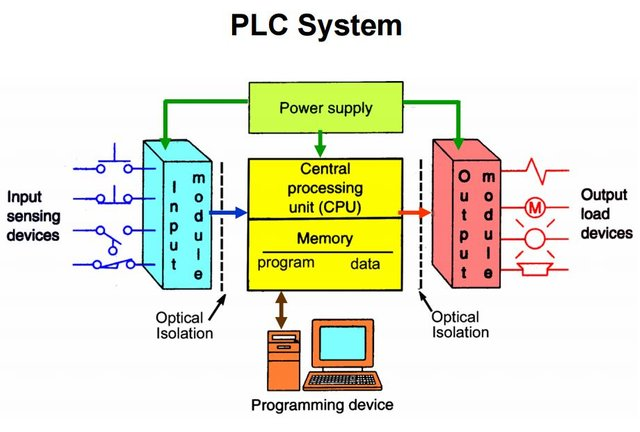
\includegraphics[ clip, trim=0.5cm 0.5cm 0.5cm 0.5cm, width=0.70\textwidth]{./images/plc.JPG}\\
	\quelle\url{https://instrumentationforum.com/t/architecture-of-plc/7059} 
	\caption{Blockdiagramm SPS}
	\label{fig:plcFigure}
\end{figure}

%\subsection{Konzept?}
\subsection{Ausgangssituation} 

Als Vorbild für dieses Projekt dient die Kleinsteuerung Easy vom Hersteller Eaton. Das Einstiegsmodell bietet hier acht Eingänge und vier Ausgänge. Das Logikprogramm, welches die Eingänge der Steuerung logisch mit den Ausgängen verbindet wird hier, auf einem kleinen Display, direkt am Gerät erstellt. Dabei stehen neben den physikalischen Ein- und Ausgängen auch Zeitfunktionen oder Zählerbausteine zur Verfügung. *Erweiterbar* Im Programmiermodus wird links einen Pluspol und rechts einen Minuspol Symbolisiert. Der anzusteuernde Ausgang, welcher obligatorisch ist, steht dabei stets ganz rechts. Der Strompfad kann nunmehr bis zum Pluspol durch gezeichnet werden, oder aber durch Sensoren unterbrochen und verzweigt werden. Aus diesem Schaltplan werden dann die booleschen Gleichungen gewonnen, die die Steuerung im Betrieb durchläuft um die Werte der Ausgänge zu bestimmen.

\begin{figure}[htbp]
	\centering
	\includegraphics[page=2, clip, trim=2.5cm 20cm 6.9cm 2.5cm, width=1.00\textwidth]{./code/GartenEasy.pdf}
	\caption{Programm einer Easy Kleinsteuerng}
	\label{fig:easyprogram}
\end{figure}

\subsubsection{Bedienoberfläche} 
Eine ähnliche Vorgehensweise ist auch in diesem Projekt geplant. Da der Raspberry Pi Netzwerkfähig ist, wurde jedoch anstatt einem Display am Gerät eine Bedienoberfläche gewählt, welche im Internetbrowser bedienbar ist. Als Basis für die Programmieroberfläche, wurde das Projekt CircuitVerse *REF* herangezogen. Hierbei handelt es sich um einen Logiksimulator, in welchem komplexe Logikschaltungen durch Drag\&Drop erstellt werden können. Das Quelloffene Projekt ist auf GitHub *REF* verfügbar und dank  der MIT *REF* Lizenz zur Erweiterung und Modifikation freigegeben. Dabei musste das Projekt vor allem durch eine Funktion ergänzt werden, um die Erstellte Logik in einem Format zu Exportieren, welche vom Backend verstanden wird. Weiterhin musste die zur Verfügung stehenden Ein- und Ausgänge dahingehend modifiziert werden, dass nur Schaltungen erstellt werden können, die auch vom Backend verstanden werden. 
Im Vorbild kann der Schaltplan auch Laufzeitinformationen wiedergeben. So wird ein (symbolisch) unter Spannung stehender Zweig als breite Linie dargestellt, während unbestromte zweige schmal gezeichnet werden. Dies Laufzeitinformationen sollen in dieser Bachelorarbeit ebenfalls dargestellt werden.
\subsubsection{Backend} 
Als Schnittstelle zwischen Hardware und Bedienoberfläche wird eine Software eingesetzt, die das vom Benutzer erstellte Logikprogramm kontinuierlich durchläuft, und somit sicherstellt, das eine Änderung an einem Eingang, der Ablauf eines Timers etc. die Werte der davon abhängigen Ausgänge entsprechend verändert. Wie dies im Vorbild der Easy Kleinsteuerung gelöst wird, bestand kein Einblick.  

\subsubsection{Hardware} 
Wie schon vorab beschrieben, bildet ein Raspberry Pi die Grundlage für dieses Projekt. Dieser bietet von Haus aus einige GPIOs, welche  dazu  verwendet werden können um Sensoren abzufragen oder um Aktoren anzusteuern. Jedoch viel die Entscheidung darauf, eine Erweiterungskarte (HAT) zu diesem Zweck einzusetzen. Dies dient erstmals zum Schutz des Raspberry Pi, zudem bietet das eingesetzte Board jedoch Leuchtdioden an den Ausgängen, sowie Taster an den Eingängen, was das Testen erheblich vereinfacht. Da der Anschluss per SPI erfolgt, können theoretisch mehrere solcher Boards parallel betrieben werden. 

\subsection{Versionsverwaltung}
Da im bisherigen Studium lediglich auf SVN als Versionsverwaltung tiefer eingegangen wurde wobei eine Versionsverwaltung für ein Projekt dieser Größe als notwendig erachtet wurde, fiel der Gedanke auf GIT. Git ist eine dezentrale Versionsverwaltung, die Notwendigkeit für einen Versionierungsserver entfällt hierdurch. Jedoch ist es in Git möglich ein- oder mehrere sogenannte Remotes hinzuzufügen. Das sind entfernte Git-Repositorys die mit dem lokalen Repository synchronisiert werden können. In der Praxis wird Git häufig eingesetzt, weshalb sich diese Bachelorarbeit als Einarbeitung anbot. Zunächst wurde ein lokales Git Repository erstellt, welches in Folge mit einem Remote-Repository auf GitHub verbunden wurde. Angedacht war ein Development-Branch und jeweils ein Feature Branch welcher nach Vollendung des entsprechenden Features in den Development Branch zurückgeführt werden soll. Darüber hinaus, soll ein Tagging erfolgen. Dabei soll für jeden Zeitbalken *WORD* im, in der vorhergehenden Projektplanung erstellten Gantt Diagramm, ein Tag erstellt werden. 

\subsection{Entwicklungsumgebung}
Ein Problem dass dieses Projekt bietet ist, dass nicht direkt auf dem Zielsystem entwickelt wird. Das hat zur Folge, dass das Programm entweder auf dem Entwicklungssystem Crosskompiliert werden muss, oder die Quelldateien auf das Zielsystem kopiert werden müssen um sie dort zu kompilieren. Da das Aufsetzen eines Crosskompilers inklusive der dazu nötigen Toolchain als zu Aufwändig erachtet wurde, blieb nur der Weg das Projekt direkt auf dem Zielsystem zu übersetzen. Um sich die Arbeit zu erleichtern wurde nach einer Entwicklungsumgebung recherchiert, die ein Übersetzen über eine SSH Verbindung zulässt. NetBeans bietet diese an, dabei wird entweder das gesamte Projekt beim Übersetzen per SSH auf das Zielsystem übertragen und dort übersetzt, oder es kann ein Mountpunkt definiert werden, an dem eine Systemfreigabe eingehängt ist (z.B. Samba-Freigabe). Im Laufe des Projektes wurde eigens dafür ein Samba Server auf dem Zielsystem installiert. Von nun an konnte also in der Entwicklungsumgebung direkt auf den Dateien des Raspberry Pi gearbeitet werden, wobei per Tastendruck eine SSH Verbindung aufgebaut wird um auf dem Zielsystem \chphl{make} auszuführen. Dabei werden sämtliche Comiler Ausgaben in einem Fenster angezeigt. Auch Debugging ist auf diesem Wege möglich.

\subsection{C++ Library LibPiFace}
Wie im vorhergenenden Abschnitt *REF* beschrieben, bildet die Erweiterungskarte PiFace Digital 2 *REF* die Grundlage für diese Bachelorarbeit. Im Lieferumfang befindet sich eine in C geschriebene Library inklusive eines Lauffähigen Tests, welche ebenfalls auf GitHub unter https://github.com/piface/libpifacedigital zu finden ist. Diese Library stützt sich wiederrum auf die Library https://github.com/piface/libmcp23s17 welche den verbauten SoC über SPI anspricht. Im Laufe der Arbeiten fiel jedoch auf, dass die C Library nicht alle benötigten Funktionen enthielt. Da der Quellcode vorlag, und die Lizensierung Veränderungen am Quellcode zulässt, lag die Überlegung nahe die benötigten Funktionen direkt in der Library zu ergänzen anstatt sie im eigentlichen Projekt unterzubringen. Weiterhin schien es auch ein erstrebenswertes Lernziel zu sein, das Erstellen und Übersetzen von statisch bzw. dynamisch gelinkten Bibliotheken kennenzulernen. Zuletzt schien es schlichtweg die Sauberste Lösung zu sein. Zunächst wurde angenommen, dass sich auch mehrere Hardwaremodule per SPI mit einem einzelnen Rasperry Pi verbinden lassen. Dies ist technisch auch möglich, so bieten die eingesetzten Boards die Möglichkeit über einen Jumper eine Hardwareadresse einzustellen. Der Hersteller bot auch die passende Hardware an, um mehrere Boards mit einem Rasperry Pi zu verbinden. Jedoch wurden diese scheinbar mangels Nachfrage aus dem Sortiment genommen. Obwohl eine Bastellösung es immer noch ermöglichen würde, ist der Aufwand hierfür sehr hoch und scheint unwirtschaftlich. Leider wurde bis zu dieser Erkentniss schon einiges an Energie darin investiert, mehrere Boards zu unterstüzen. Dies ist auch der Grund wieso ein Objektorientierter Ansatz in C++ gewählt wurde - eine Instanz für jedes Harwaremodul. Ein weiterer Grund war, dass die Anwendung ohne Caching nicht performant genug war. Das heißt die zeitliche Lücke zwischen einer Änderung an einem Eingang bis zu dessen Auswirkung am Ausgang war deutlich spürbar. Dafür wurden Methoden vorgesehen, um das Caching ein un auszuschalten - bei eingeschaltetem Caching verändern die Methoden um Bytes und Bits zu schreiben, lediglich den Wert einer Instanzvariable. Derzeit muss das leeren des Chaces explizit mittels Aufruf der Methode \textit{flush()} erfolgen. Über ein Automatisches verfahren wurde nachgedacht, jedoch erwies sich der manuelle Aufruf als einfacher. 

    
\clearpage

    \section{Umsetzung}\label{kap:ums}

\todo{Struktur Umsetzung einfügen }

\subsection{Parsen von Logikausdrücken}\label{kap:ums:parsing}
Das Ziel dieses Projektes ist es, dass die Ausgänge der Steuerung in Abhängigkeit von Eingängen wie physikalischen Eigängen oder zum Beispiel Timer-bausteinen ein beziehungsweise ausgeschaltet werden. Dafür ist in einer Textdatei für jeden Ausgang eine Zeile vorgesehen. Eine Zeile beginnt hierbei mit dem zu definierenden Ausgang, also zum Beispiel Ho1, worauf ein Gleichheitszeichen zu folgen hat. Der gesamte Ausdruck hinter dem Gleichheitszeichen wird zur Laufzeit des Programms durchlaufen, wobei jedes vorkommende Paar von [ und ] durch eine Null oder eine Eins ersetzt. Innerhalb der Klammern, findet sich gleich genau wie bei dem Bezeichner vor dem Gleichheitszeichen, die jeweilige Bezeichnung der Abhängigkeit. Lautet die Zeile also etwa Ho0= [Hi0] \& [Hi1] so wird die Komplette erste Klammer durch den Wert von Hi0 ersetzt, wärend die zweite Klammer  durch den Wert von Hi1 ersetzt wird. Daraus ergibt sich dann, vorausgesetzt Hi0 und Hi1 sind im Zustand \chphl{Ein}, Ho0= 1 \& 1. Das für den Leser offensichtliche Ergebnis dieser Gleichung ist 1 oder \chphl{true}. Jedoch gestaltet sich eine programmatische Lösung des Problems als deutlich komplexer. Denn sobald mehr als drei Ausdrücke im Spiel sind, müssen wie bei klassischer Mathematik Rechenregeln befolgt werden. Punkt vor Strich sowie die Beachtung von Klammern. Dabei kann ein Ausdruck beliebig Komplex sein. Eine Rechersche nach Ansätzen führte zu Stackoverflow. (Siehe  
\footnote{Abr. 11.03.2019 \url{https://stackoverflow.com/questions/8706356/boolean-expression-grammar-parser-in-c/8707598\#8707598}}
 und  \footnote{Abr. 11.03.2019 \url{http://coliru.stacked-crooked.com/a/c40382620fb75b75}}) Dieser Ansatz löste genau das Problem und wurde somit in das Projekt übernommen. 
%
\subsection{Automatische Prüfung von Abhängigkeiten}\label{kap:ums:abh}
Ein Problem was sich mit dem Einbinden der Lösung zum Parsen der Logikausdrücke ergab, war die Abhängigkeit zu Boost. Auf dem Desktop Computer auf dem die Lösung getestet wurde, konnte das Projekt dank installiertem boost Paket ohne Probleme übersetetzt werden. Da es sich bei dem  Zielsystem jedoch um eine ARM Architektur handelt, musste der code dort Übersetzt werden. In den Paketquellen des dort installieren Raspian, ist jedoch eine ältere Version des Boost Pakets hinterlegt, was dazu führt dass Boost manuell heruntergeladen und gebaut werden muss. Obwohl sich dieses Problem im Laufe der Zeit durch aktualisierung des Paketes in den Paketquellen von Raspian von selbst lösen wird, muss dennoch geprüft werden ob die installierte Version den Ansprüchen genügt. Hierfür wurde ein Bash script erstellt, welches auch alle weiteren abhängigkeiten Prüft und gegebenenfalls installiert. Dazu zählen auch die in *REF* erwähnten Bibliotheken um die Hardware anzusprechen und wie in *REF* erwähnt der verwendete Kompiler. 
 
\subsection{Benamungsschnema}\label{kap:ums:banamsung}
Nachdem die Auswertung beziehungsweise das Parsing der Logikausdrücke funktionierte, sollte auch die Auswertung der Bezeichner automatisiert werden. Ein Benamsungsschema wurde dabei schon vorher erdacht. Es besteht aus einem führenden Großbuchstaben, gefolgt von einem Kleinbuchstaben und einer Zahl. Dabei wird der führende Buchstabe als Kanal bezeichnet, der zweite als Entität und die Ziffer als Pin-Nummer. So könnte zum Beispiel der Buchstabe \chphl{H} den Kanal Hardware beschreiben, welcher  wiederrum die Entitäten \chphl{i} für Input und \chphl{o} besitzt, welche jeweils ein Byte, also 8 Bits oder Pins haben. 

\subsection{Klassenstrukrur und Kanäle}\label{kap:ums:klassen}
Im Programm werden die zuvor beschriebenen Kanäle von einem Abkömmling der Basisklasse \chphl{IO\_Channel} (siehe Abb. \ref{img:classIOChannel}) repräsentiert. Wobei jeder Kanal als Eigenschaft eine Map mit Entitäten führt, welche durch Objekte des Typs \chphl{Channel\_Entity} (siehe Abb. \ref{img:classChannelEntity}) repräsentiert werden. Eine Entität wiederum weiß, wie groß ihre Breite ist, also wie viele Bits sie hat und ob sie nur lesbar oder auch beschreibbar ist. Eine weitere Klasse \chphl{IO\_Channel\_AccessWrapper} (siehe Abb. \ref{img:classAgregation}) bündelt alle vorhandenen Kanäle inklusive der jeweiligen Entitäten. Zudem erleichtert Sie mittels Überladung der Array-Operatoren den Zugriff. Ein Zugriff ist dann wie in Listing \ref{code:chnlAccess} gezeigt wird möglich. Dazu müssen die Entsprechenden Kanäle vorher wie in Listing \ref{code:chlnInit} zu sehen initialisiert und einer Instanz der Klasse \chphl{IO\_Channel\_AccessWrapper} übergeben werden. Der für den späteren Zugriff auf den Kanal nötige Buchstabe, wird in diesem Zuge festgelegt, während die Buchstaben der untergeordneten Entitäten Bestandteil des jeweiligen Kanals sind und dementsprechend dort definiert werden. 


\begin{listing}[H]
	\inputminted[numbersep=1pt,fontsize=\scriptsize,frame=single, firstline=364,lastline=369]{c}{./code/main-klassenstruktur.cpp}
	\caption{Initialisieren der Kanäle und Entitäten}
	\label{code:chlnInit}
\end{listing}


\begin{listing}[H]
	\inputminted[numbersep=1pt,fontsize=\scriptsize,frame=single, firstline=415,lastline=416]{c}{./code/main-klassenstruktur.cpp}
	\caption{Zugriff auf Kanal und Entität exemplarisch}
	\label{code:chnlAccess}
\end{listing}


\begin{figure}[H]
	\begin{center}
		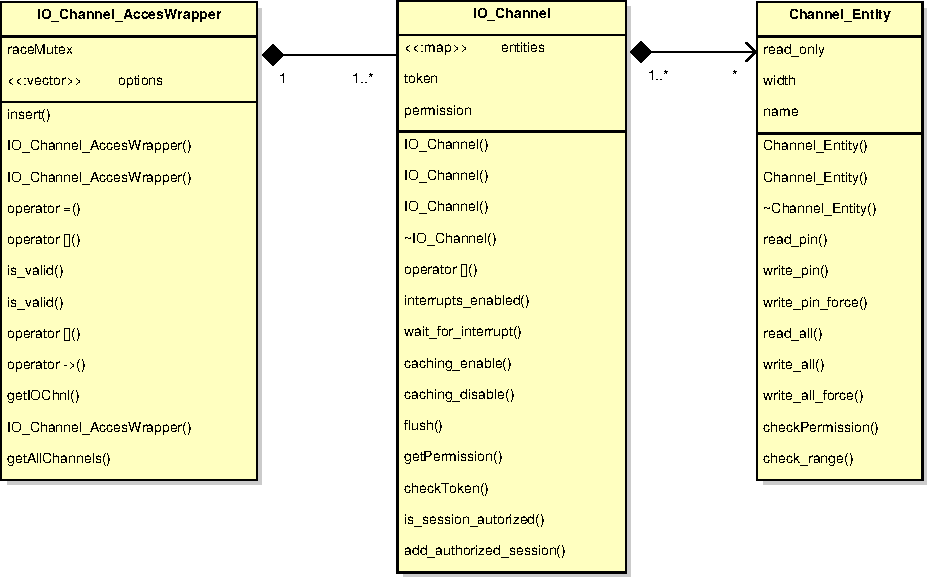
\includegraphics[width=0.95\textwidth ,clip]{./code/Aggregation.pdf}
		\caption{Klassendiagramm Aggregation der Klassen}
		\label{img:classAgregation}
	\end{center} 
\end{figure}	
Zu sehen ist die Aggregation zwischen dem \chphl{IO\_Channel\_AccessWrapper} den Kanälen \chphl{IO\_Channel} und den Entitäten \chphl{Channel\_Entity}. Alle Kanäle werden von dem  \chphl{IO\_Channel\_AccessWrapper} zusammengefasst. Ein Zugriff erfolgt ausschließlich über diesen Weg. 


\begin{figure}[H]
	\begin{center}
		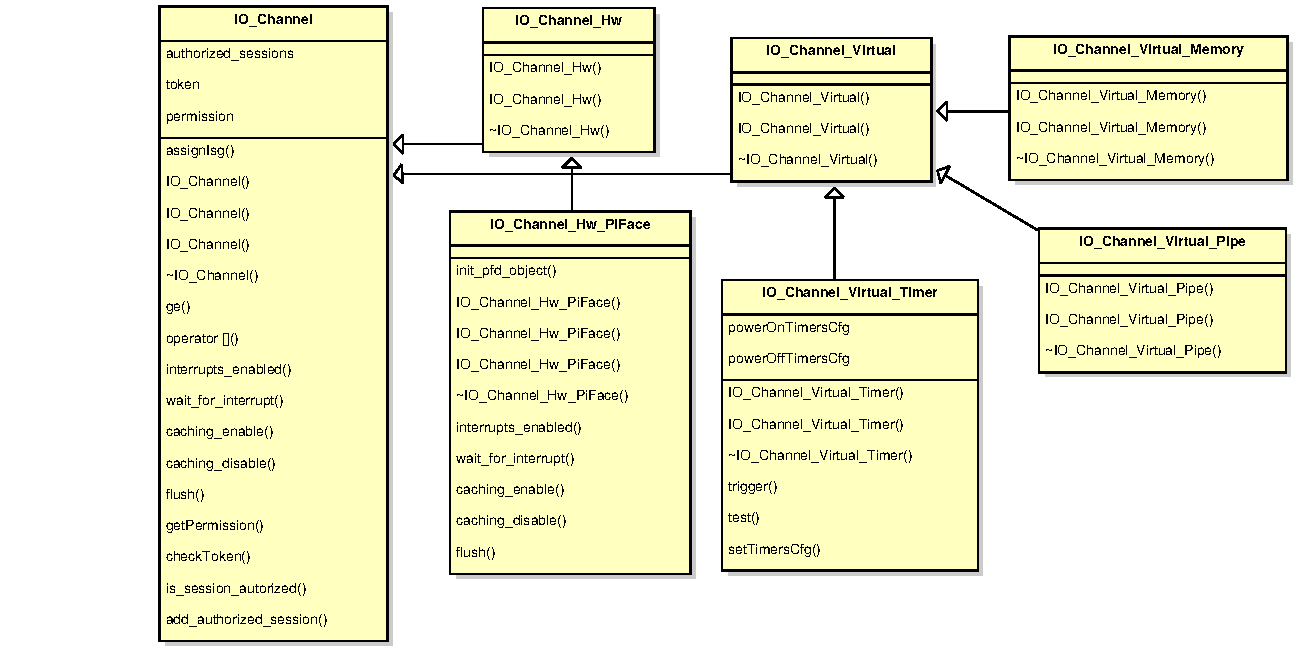
\includegraphics[width=0.95\textwidth ,clip]{./code/IOChannel.pdf}
		\caption{Vererbungshierarchie der Basisklasse IOChannel}
		\label{img:classIOChannel}
	\end{center} 
\end{figure}	

\begin{figure}[H]
	\begin{center}
		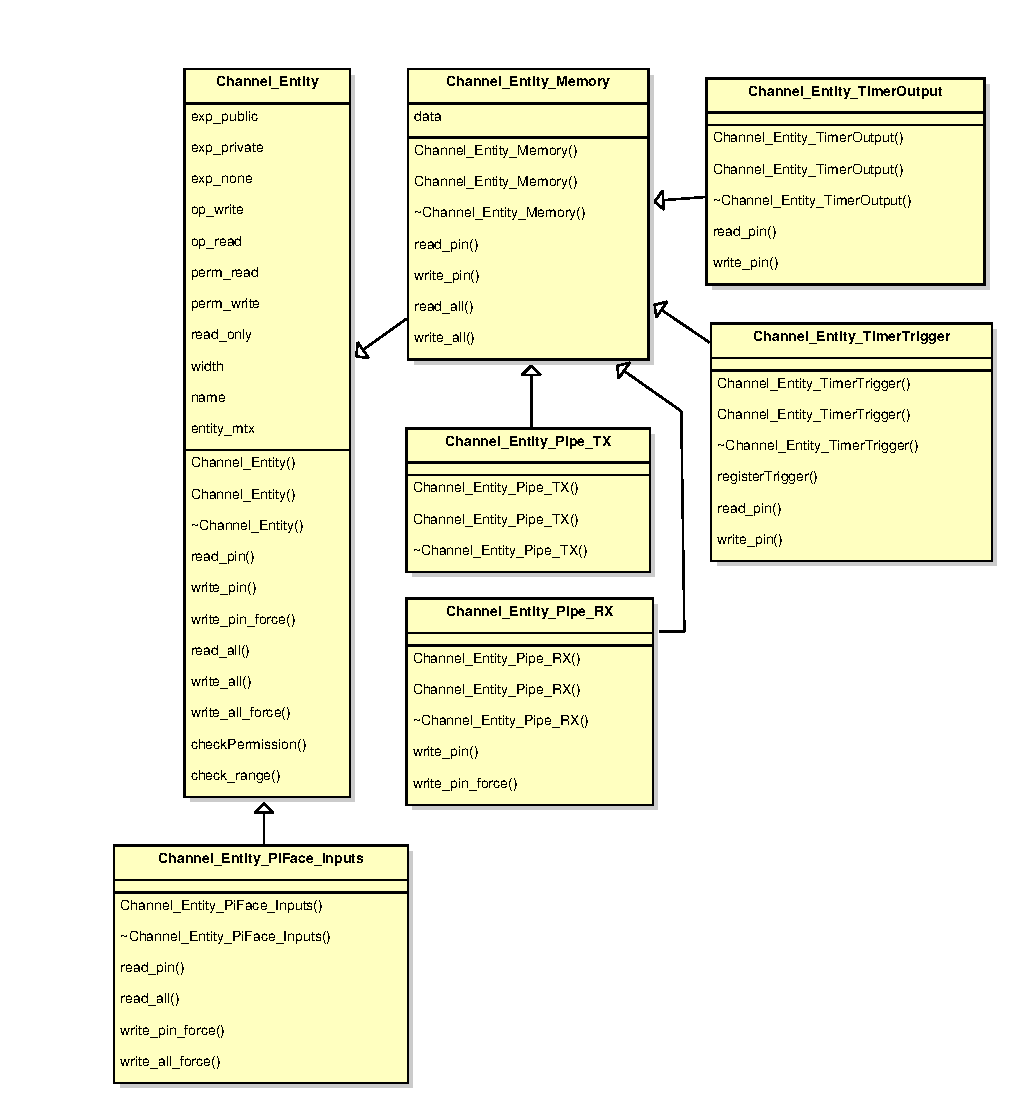
\includegraphics[width=0.95\textwidth ,clip]{./code/ChannelEntity.pdf}
		\caption{Vererbungshierarchie der Basisklasse ChannelEntity}
		\label{img:classChannelEntity}
	\end{center} 
\end{figure}	

Die Entitäten erben von der Basisklasse Entity. Sie überschreiben Methoden um lesend oder schreibend, entweder auf den gesamten Inhalt auf einmal oder Bitweise auf den Inhalt zuzugreifen. Dafür sind die Methoden read\_pin, write\_pin beziehungsweise read\_all und write\_all vorgesehen. 



\subsubsection{Hardware Kanäle}\label{kap:ums:hwchannels}
Der Wohl wichtigste Kanal ist der Hardware Kanal. Die Klassenstruktur in Abb. \ref{img:classIOChannel} zeigt, dass alle Kanäle eine gemeinsame Basisklasse haben. Der Hardware Kanal ist eine Spezialisierung der Basisklasse, welche spezifische Funktionen für die Entsprechende Hardware beherbergt. So finden sich hier Methoden zur Steuerung des Caching sowie ein blockierender Aufruf, welcher auf einen Interrput an der Hardware reagiert. Die Funktionen für den schreibenden und lesenden Zugriff auf die Ein- und Ausgänge der Hardware, sind in Entitäten gekapselt. Für eben jenen Zweck existieren zwei Spezialisierungen der \chphl{Channel\_Entity} (siehe Abb. \ref{img:classChannelEntity}) Basisklasse, welche für den Zugriff mit \chphl{i} für den Eingang (input) beziehungsweise \chphl{o} für den Ausgang (output) referenziert werden.   

\subsubsection{Merker Bausteine}\label{kap:ums:memorychannel}
Die erste Erweiterung, welche wie in Abb. \ref{code:chlnInit} zu sehen mit dem Buchstaben M referenziert wird, sind Memory Bausteine. Da ein Memory Baustein nicht richtungsorientiert sind, das heißt es existiert keine Eingangs oder Ausgangsgröße, wurde hier vom Benamsungsschema für Entitäten  abgewichen. Eine Referenzierung ist hier mittels eines oder mehrerer Buchstaben geplant. Somit bietet ein Merker Baustein Platz für 8 Zustandswerte pro verwendeter Entität. Bislang ist lediglich die Entität \chphl{a} angelegt, wobei geplant ist die Anzahl an Buchstaben beziehungsweise Entitäten durch einen Konstruktorparameter nach Außen zu führen, womit die Anzahl wie in Abb. \ref{code:chlnInit} zu sehen beim Einfügen bestimmt werden könnte, oder in einem weiteren Schritt in eine Konfigurationsdatei exportiert werden kann. 

\subsubsection{Timer Bausteine}\label{kap:ums:timerchannel}
Timer Bausteine waren die wohl komplexesten Bausteine. Eine Verzögerung im Programmablauf bedeutet entweder ein blockieren, was aber bedeuten würde, dass das Programm in dieser Zeit auch nichts anderes tun kann und somit nicht auf Ereignisse reagieren kann. Die andere alternative ist Multithreading, also das Einführen von Parallelen Handlungssträngen, welche weitere Probleme bringen. So muss zum Beispiel beim Zugriff auf gemeinsam genutzte Ressourcen dafür sorge getragen werden, dass nicht gelesen wird während gerade geschrieben wird. Des weiteren musste die Hauptschleife überarbeitet werden. Bislang wurde die Programmlogik bei jedem eintreten eines Hardware-Ereignisses genau einmal durchlaufen. Jedoch muss die Programmlogik nun auch durch Ablauf eines Timers erneut durchlaufen werden. Gelöst wurde dies mithilfe einer Binären Variable als Schalter, welche zusammen mit eines Mutex zur Vermeidung von gleichzeitigem Zugriff, und einer Condition Variable zur Benachrichtigung des Hauptprozesses, in die Klasse \chphl{iterationSwitchGuard} gekapselt wurde. 
Ein Timerbaustein (mehrere sind Theoretisch möglich), bietet 8 Konfigurierbare Timer. Dabei gibts es eine Entität um einen Timer auszulösen \chphl{t} (Trigger) und eine Entität, welcher als Ausgang fungiert \chphl{o} (Output). So ergibt sich in der Programmlogik die selbe Syntax, welche sich auch bei Hardwarekanälen bietet: Ein explarisches triggern des Timers 3 würde erfolgen, indem eine Zeile der Logikdatei mit \chphl{Tt3=} beginnt. Eine Verwendung des Ausgangswertes desselben Timers, würde durch integrieren des Bezeichners \chphl{[To3]} in die Logikzuweisung eines anderen Bezeichners erfolgen. Die Parametrisierung des Timers erfolgt durch einbinden einer Konfigurationsdatei (siehe Listing \ref{code:timersConf}) hierbei lassen sich für jeden Timer eine Einschaltverzögerung sowie eine Ausschaltverzögerung definiert werden. Jeder Wert ungleich null bewirkt eine Verzögerung, eine gleichzeitige Nutzung von Ein und Ausschaltverzögerung ist möglich. Werte gleich null bewirken eine sofortige Änderung am Ausgang, sobald sich der Eingangswert verändert. Beim Einlesen der Konfiguarionsdatei werden sämtliche Leerzeichen entfernt. Zudem kann mit einem Semikolon \chphl{;} oder einer Raute \chphl{\#} ein Kommentar eingeleitet werden, welches alle restlichen Zeichen der Zeile beim Einlesen entfernt. Die Verzögerungszeiten sind in Millisekunden anzugeben, wobei die Reihenfolge der nicht sukzessive erfolgen muss. Der Maximalwert beläuft sich auf 4.294.967.295, was die größte in unsignes long darstellbare Zahl ist und umgerechnet etwa 49 Tagen entspricht. 
\begin{listing}[H]
	\inputminted[numbersep=1pt,fontsize=\scriptsize,frame=single, firstline=14,lastline=25]{c}{./code/timers.conf}
	\caption{Beispiel der Timer Konfigurationsdatei}
	\label{code:timersConf}
\end{listing}


\subsubsection{Virtuelle Kanäle}\label{kap:ums:virtualchannel}
Virtuelle Kanäle sind ein Konzept dass die Kommunikation der Steuerung mit entfernten Endpunkten ermöglichen. Ein Virtueller Kanal ist hierbei lediglich ein veränderter Memory Baustein, welcher entgegen entgegen anders als ein normaler Memory Baustein wieder richtungsorientiert ist. Das heißt es gibt eine Eingangs-Entität und eine Ausgangs-Entität. Hierbei muss beachtet werden, dass die Perspektive so gesetzt ist, dass ein Eingang die extern empfangenen Daten beinhaltet. Während in den Ausgang geschrieben wird. Die Gegenseite bildet der in *REF* beschriebene WebSocket Server, beziehungsweise was auch immer die Gegenseite bildet. Das kann das WebFrontend *REF* dieses Projektes sein, oder auch jeder andere WebSocket fähige Client. Angedacht ist auch die Implementierung eines WebSocket Clients in das Backend, womit sich zwei Einheiten verbinden ließen. 


\subsection{Laden der Programmlogik aus Datei}\label{kap:ums:logicOutsource}
Das Logikprogramm wurde im nächsten Schritt in eine Textdatei ausgelagert. Sie soll künftig von der grafischen Benutzeroberfläche automatisch erstellt werden können, kann aber nach wie vor auch von Hand erstellt werden. Die Datei enthält einen Ausgang pro Zeile, gefolgt von einem Gleichheitszeichen und den Abhängigkeiten. Zeichen die auf ein Semikolon folgen, werden dabei als Kommentar gewertet und ausgelassen. Sie wird bei Programmstart eingelesen und verbleibt dann im Speicher. Zum Speichern der Daten wird ein \chphl{Vector} benutzt, welcher für jede Zeile der Logikdatei einen weiteren Eintrag erhält. Da vor einem Gleichheitszeichen lediglich ein Ausgang stehen darf (z.B. \ref{softLogic} Zeile 1: \chphl{Ho0}), ist somit jeder Eintrag des Vectors die Definition genau einer Abgeschlossenen Zuweisung. Bei Mehrfacher Definition eines Ausgangs, überschreibt die spätere Definition die vorangegangene. 

\begin{listing}[H]
	\inputminted[numbersep=1pt,fontsize=\scriptsize,frame=single, firstline=29,lastline=36]{c}{./code/logic.conf}
	\caption{Beispiel der Programmlogik Datei}
	\label{code:softLogic}
\end{listing}


\subsubsection{Erneutes Laden der Logik zur Laufzeit}\label{kap:ums:reloadConf}
Zum erneuten einlesen der Logik, wurde ein Signalhandler vorgesehen, welcher auf das Signal SIGUSR1 hört. Die entsprechende Funktion ließt dann die Logikdaten erneut ein und überschreibt damit die vorherige Version im Speicher. Damit muss die Steuerung nicht neu gestartet werden und ermöglicht das Steuerungsprogramm zur Laufzeit zu verändern.


\subsection{Hauptschleife und Iterationslogik}\label{kap:ums:mainloop}
Das Logikprogramm liegt nun im Speicher und das Programm betritt die Hauptschleife. Doch treibt ein einfaches polling die Auslastung des Prozessors unnötig nach oben. Nun könnte nach jedem Durchlauf eine gewisse Zeit gewartet werden, bevor eine neue beginnt. Doch das verringert die Reaktionszeit der Steuerung. Die beste Lösung findet sich direkt im Treiber des PiFaceDigital. Hier bietet sich eine Funktion, die bis zum Eintreten einer Veränderung der  Eingangswerte blockiert. Intern Eingesetzt wird hier ein Epoll, welcher einen File descriptor auf einen der GPIOs des Raspberry Pi überwacht und diesen somit als Interrupt Kanal nutzt. 


\subsection{Logik Prozessor}\label{kap:ums:logicProcessor}
Den Kern des Projektes bildet der in \autoref{code:logicEngine} gezeigte Logikprozessor. Es ist eine Methode, welche den in \autoref{kap:ums:logicOutsource} geladenen Logik-Vektor zeilenweise durchläuft. Im ersten Schritt wird die Zeile nun auf Vorhandensein eines Gleichheitszeichens hin überprüft (\autoref{code:logicEngine} Zeile \ref{codeline:split}). Eine Zeile ohne Gleichheitszeichen wird hierbei schlicht verworfen. Andernfalls wird zunächst der Teil vor dem Gleichheitszeichen näher untersucht. Dabei wird sichergestellt dass der Bezeichner aus drei Zeichen besteht, wobei die ersten beiden alphabetisch und der letzte numerisch sein muss. Diese drei Teile werden dann (Zeile \ref{codeline:charSeperateBegin}-\ref{codeline:charSeperateEnd}) für die weitere Verarbeitung gespeichert. Der fertig ausgewertete Teil nach dem Gleichheitszeichen, auf dessen Verarbeitung nachfolgend noch etwas genauer eingegangen wird und der nunmehr entweder \texttt{0} oder \texttt{1} ist, wird dem entsprechenden Kanal nun zugewiesen. Wie in \autoref{code:logicEngine} Zeile \ref{codeline:equation} zu sehen, wird nun eine Instanz \texttt{chnl} der Klasse \texttt{IO\_Channel\_AccessWrapper} für den eigentlichen Zugriff auf die Ressource verwendet. Zuvor müssen jedoch die vorher gespeicherten Teile des Bezeichners eingefügt werden verwendet. (Siehe \autoref{kap:ums:klassen}\chphl{ \nameref{kap:ums:klassen}}). 
Zudem wird dem Bezeichner in diesem Zuge ein Wert zugewiesen. Um diesen zu erhalten muss nun die Gleichung gelöst werden. Diese beinhaltet ebenfalls Bezeichner, welche vom Funktor \texttt{replaceIdentifier} durch dessen aktuellen Wert ersetzt wird. Zurück gegeben wird ein String, welcher nun nur noch aus Binärzahlen, arithmetischen Operatoren (\& für und bzw. | für oder) und Klammern besteht. Die eigentliche Lösung der Gleichung erfolgt dann mittels eines Funktionsaufrufes auf einen in Boost Spirit geschriebenen Parser (siehe Unterabschnitt \chpref{kap:ums:parsing}). 
\begin{listing}[H]

	\inputminted[numbersep=1pt,linenos=true, mathescape, numbers=left, fontsize=\scriptsize,frame=single, firstline=186,lastline=222]{c}{./code/main-klassenstruktur.cpp}
	\caption{Logik Engine}
	\label{code:logicEngine}
\end{listing}
\subsection{WebSocket Server}\label{chp:ums:websockserver}
\subsubsection{Basis}
Um die Steuerung mit der Außenwelt zu Verbinden wurde ein WebSocket (siehe \ref{chp:grdlgn:webSocket}) Server in das Backend integriert. Als Basis hierfür diente das Beispiel, welches von Vinnie Falco im  Rahmen eines Vortrages auf der \texttt{CppCon 2018} erstellt wurde \cite{URL:WebSocketCppCon}. Die Funktion dieses Beispiels ist das Bereitstellen  eines WebSocket Chatservers. Dieser baut auf einem rudimentären HTTP Server auf und ist deshalb in der Lage auch normale HTTP Anfragen zu beantworten. Auf diesem Wege erhält der Webbrowser des Clients die HTML Webseite, in welche gleichzeitig auch der JavaScript Chat-Client enthalten ist der letztendlich die direkte Verbindung zum WebSocket Server aufbaut. Nachdem die Verbindung erfolgreich herstellt wurde, kann der Benutzer Texteingaben tätigen und diese an den Server senden, welcher diese dann an alle verbunden Clients verteilt. Da es nun relativ einfach umsetzbar ist, anstatt Text auch andere Formate wie etwa JSON über diesen Server an die Clients zu senden, schien dieses Beispiel eine ideale Grundlage zu sein. So könnte anstatt Text ein JSON mit dem Status der Ein- und Ausgänge der Steuerung an die verbundenen Clients verteilt werden, welche diese dann mit einer JavaScript Anwendung so umsetzen, dass der Status der Ein- und Ausgänge visuell dargestellt werden. Zudem ist über diesen Kommunikationskanal auch ein Schreibzugriff denkbar. So könnte ein symbolisch dargestellter Schalter im Frontend beim Anklicken per JavaScript Funktion einen Befehl an das Backend senden, welches diesen dann ausführt. 
\subsubsection{Erweiterung}
Das vorher erwähnte Beispiel wurde in einem ersten Schritt in einen Unterordner des Projektes verschoben und das CMake-File dahingehend geändert, das anstatt eines eigenen Executables eine Library gebaut wird, welche dann vom Grundprojekt verwendet wird. Das Unterprojekt wurde zudem als Abhängigkeit deklariert sodass es beim bauen des Hauptprojektes automatisch neu gebaut wird, sofern sich Änderungen im Unterprojekt ergeben haben. Die einfachste Erweiterung war es, die schon vorhandene \texttt{broadcast} Funktion zu verwenden, um bei einer Änderung an den Ein- und Ausgängen eine Nachricht an alle verbundenen Clients zu senden. Da jedoch immer nur eine Nachricht gleichzeitig gesendet werden kann, wurde eine \texttt{Queue} verwendet, welche die Nachrichten sammelt, und diese dann  nacheinander zustellt. Im nächsten Schritt wurden eingehende Nachrichten nun nicht mehr bloß eins zu eins an die \texttt{broadcast} Methode übergeben, und damit an alle Clients weitergeleitet. Stattdessen mündeten diese nun in eine weitere \texttt{Queue}: \chphl{Command-Queue}. Eingehende Nachrichten sollen damit gesammelt werden um die darin enthaltenen Befehle auszuführen.
\subsubsection{Zugriffsbeschränkung}
Um zu verhindern das jeder Client nun unkontrolliert vollen Zugriff auf alle Kanäle der Steuerung erhält, wurde daraufhin ein Konzept für die Zugriffsbeschränkung erarbeitet. Dafür wurden zwei Benutzerrollen eingeführt. \texttt{public} und \texttt{private}. Sie gelten für jeden Kanal und jeden Client individuell. Dafür besitzt jeder Kanal ein \texttt{private\_token}. Authentifiziert sich ein Benutzer mittels \texttt{auth:<Kanal>:<Token>} für den Kanal, so wechselt er für diesen Kanal in die Rolle \texttt{private}. Da jeder Kanal aus mehreren Entitäten besteht, besitzt nun jede dieser Entitäten die Eigenschaften \texttt{expose\_read} und \texttt{expose\_write}. Zulässige Werte hierfür sind jeweils \texttt{public} \texttt{private} oder \texttt{none}. Bei Zugriff auf den Kanal bzw. die Entität wird nun darauf geprüft ob der Benutzter \textbf{mindestens} die eingetragene Berechtigung hat. Nehmen wir zum Beispiel den Kanal Hardware \chphl{H}. Dessen Entitäten \texttt{i} für die Eingänge und \texttt{o} für die Ausgänge haben beide \texttt{expose\_read} auf \texttt{private} gesetzt. Das \texttt{private\_token} ist mit \texttt{top-secret-123} definiert. Ein Verbundener Client müsste sich nun erst mit dem Befehl \texttt{auth:H:top-secret-123} für den Kanal authentifizieren, bevor er Statusinformationen über die Entitäten dieses Kanals erhält. Wäre \texttt{expose\_read} auf \texttt{public} gesetzt, würde er diese Informationen ohne vorherige Authentifikation erhalten. Anders herum, würde derr wert \texttt{none} bedeuten, dass niemand - nicht einmal ein Authentifizierter Client - Statusinformationen zu dieser Entität erhält. Listing \ref{code:Jsonresponse} stellt ein typisches Statusupdate der privaten Entitäten \texttt{Qo} und \texttt{Qi} dar, darauf folgt das Update aller Entitäten, die als \texttt{public} definiert wurden.  
\begin{code}
	\captionof{listing}{JSON Status Update von privaten und öffentlichen Entitäten}
	\label{code:Jsonresponse}
\begin{minted}
	[
	frame=lines,
	framesep=2mm,
	baselinestretch=1.2,
	fontsize=\footnotesize,
	linenos
	]
	{c}
{"Qo" : 4, "Qi" : 1}
{"Po" : 170, "Pi" : 4, "Ho" : 0, "Hi" : 6}
\end{minted}
\end{code}

\subsection{Benutzeroberfläche}
\todo{Grafik Erstellen}
 \begin{figure}[H]
	\begin{center}
		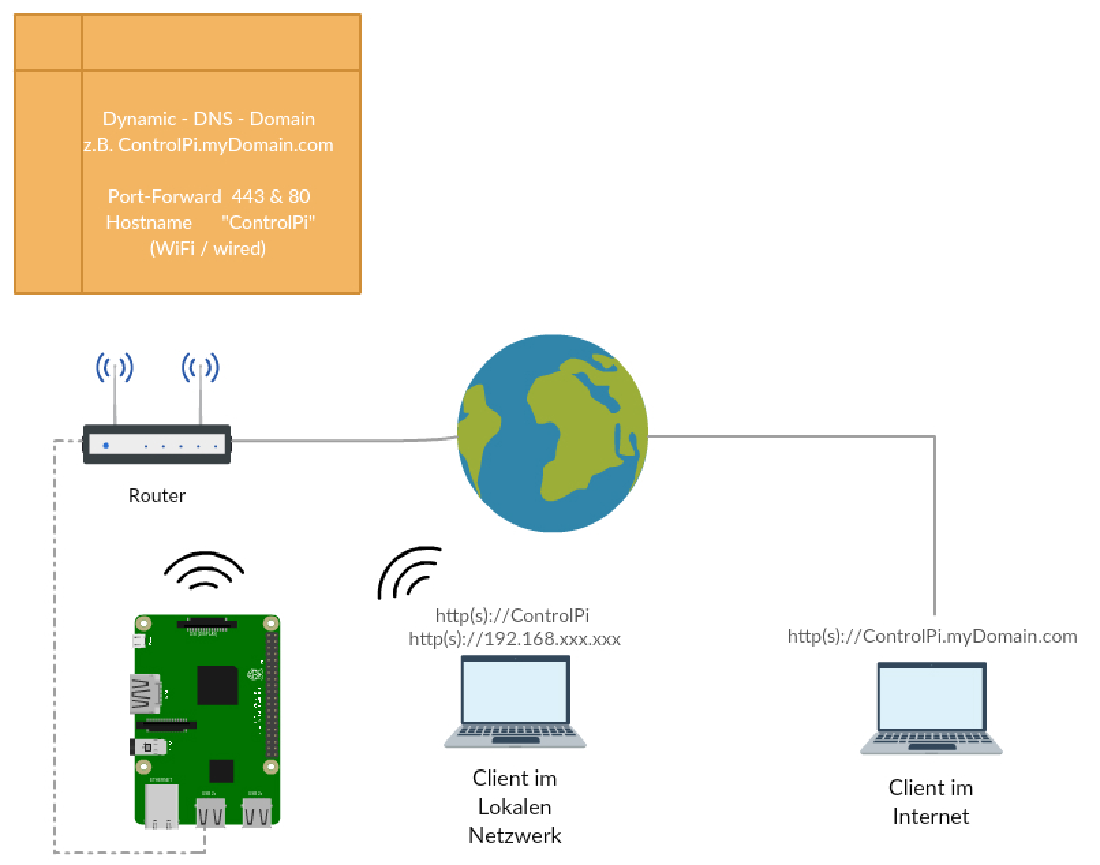
\includegraphics[width=0.75\textwidth ,clip]{./images/IFTTT.pdf}
		\caption{Zugriff auf die Weboberfläche}
		\label{img:externalAccess}
	\end{center} 
\end{figure}

\begin{figure}[H]
	\begin{center}
		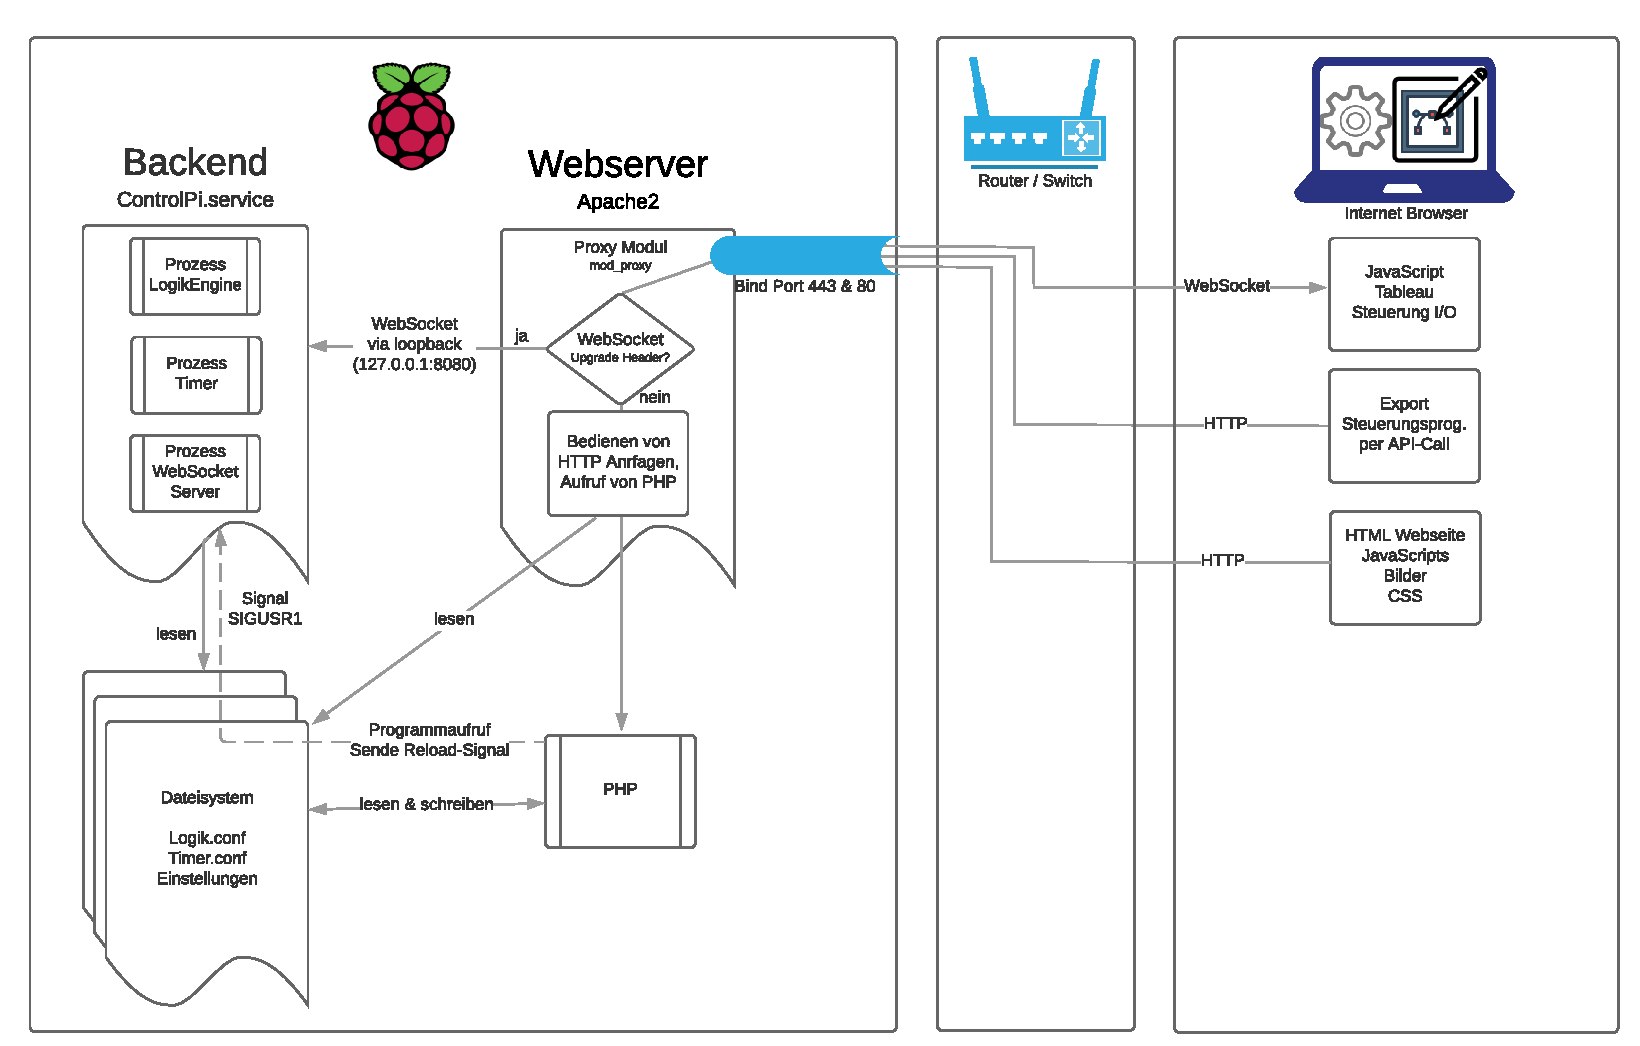
\includegraphics[width=0.9\textwidth ,clip]{./images/BackendFrontend.pdf}
		\caption{Networking Übersicht}
		\label{img:externalNetworking}
	\end{center} 
\subsubsection{Übersicht Komponenten}
Die eigentliche Anwendung ist Hauptsächlich in HTML und JavaScript und wird im Browser des Benutzers ausgeführt. Um die Benutzeroberfläche mit dem Rest der Anwendung kommunizieren zu lassen, bedarf es mehrerer Komponenten. Obwohl der Hauptteil der Anwendung über JavaScript Websockets eine direkte Verbindung vom Browser zum Backend herstellt, wird als direkte Schnittstelle zum Browser ein Apache2 Webserver eingesetzt. Dieser wird um das Proxy-Modul modproxy erweitert was es ermöglicht an das Backend gerichtete Anfragen mit dem WebSocket Header auf die lokale loopback Adresse \texttt{127.0.0.1} weiterzuleiten, während alle sonstigen Anfragen vom Webserver direkt beantwortet werden können. Zum einen wird hierdurhc die Konfiguration von Verschlüsselten Verbindungen über SSL und den Abruf der dazu nötigen Zertifikate erheblich vereinfacht, denn einige Zertifizierungs-Anbieter wie zum Beispiel Let's Encrypt *REF* bieten extra auf Apache zugeschnittene Scripte, die ebendies fast vollständig Automatisieren. Zum anderen ist es so möglich die Auslieferung der HTML und JavaScript Quellen an den Webserver zu delegieren, anstatt bei einer eigenen Implementierung Sicherheitslücken und Performance-Probleme zu riskieren. Weiterhin ermöglicht es dieser Ansatz auch PHP Scripte zu verarbeiten, dies wird zum Beispiel eingesetzt um Konfigurationsdateien vom Browser auf dem Server abzulegen, oder durch dem Backend Signale zu senden wenn es die Logikdatei erneut einlesen soll.
\subsubsection{Apache Webserver}

\end{figure}
\subsubsection{JavaScript Anwendung}
\subsubsection{Logik Editor CircuitVerse}
Die Wahl für einen Graphischen Logikeditor fiel auf den mit der MIT Lizenz gekennzeichneten Editor CircuitVerse *REF*. Die Lizenzierung gestattet es, das Programm zu verändern und weiter zu verbreiten. Der in \autoref{img:circuitVerseBasic} gezeigte Screenshot, zeigt den Aufbau des Editors. Im linken Abschnitt kann dabei zwischen verschiedenen Bauteilen gewählt werden, welche dann per Drag \& Drop auf die rechts daneben befindliche Zeichenfläche gezogen werden können. Grüne Punkte kennzeichnen dabei die Anschlussknoten, welche dann wiederum durch ziehen mit gehaltener linker Maustaste miteinander verbunden werden können. CircuitVerse bietet überdies die Möglichkeit, die erstellte Zeichnung in einem eigenen Format zu  speichern, sowie sie als Grafik zu exportieren. Des weiteren gibt es die Möglichkeit eine Zeichnung anhand einer Logiktabelle automatisch erstellen zu lassen. 

\begin{figure}[H]
	\begin{center}
		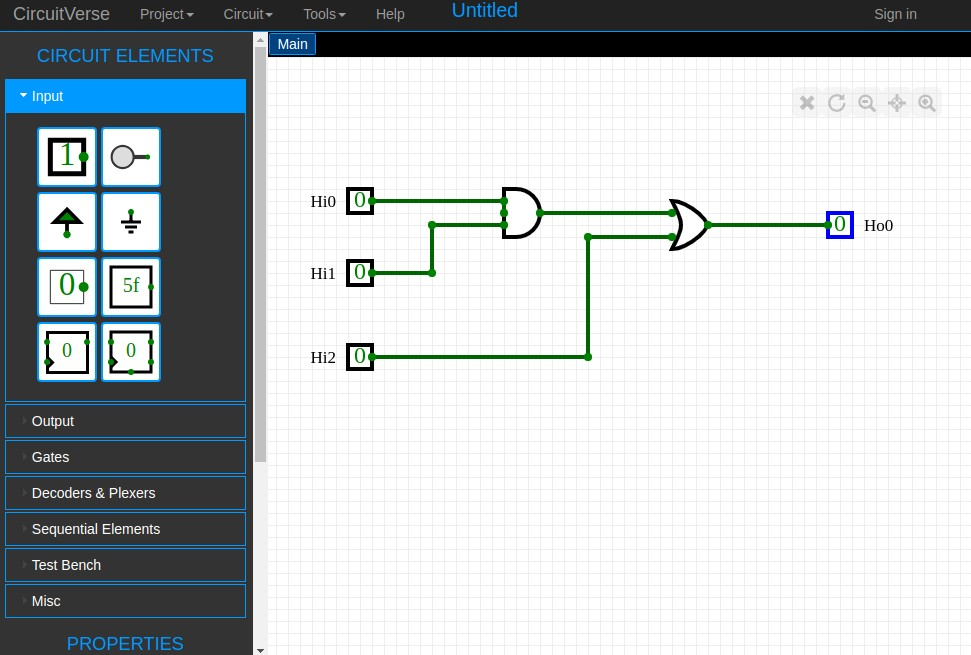
\includegraphics[width=0.65\textwidth ,clip]{./images/circuitverse.jpg}
		\caption{Screenshot einer Logikschaltung in CircuitVerse}
		\label{img:circuitVerseBasic}
	\end{center} 
\end{figure}	

\paragraph{Erweiterung für den Export}\label{par:erw}
 Eine Erweiterung von CircuitVerse ist nötig, um die gezeichnete Logikschaltung in ein Format umwandeln zu können, welches vom Backend verstanden wird. Weiterhin muss das Benamsungsschema (siehe \chpref{kap:ums:banamsung}) eingebracht werden. Letztlich muss auch die Bauteile-Auswahl auf jene Bauteile reduziert werden, welche auch tatsächlich in der Steuerung verfügbar sind. \chpref{kap:ums:logicOutsource} beschriebt das Format der Datei, die letztlich aus einer gezeichneten Logikschaltung gewonnen werden soll. CircuitVerse verwendet für die Speicherung der Schaltung eine JSON-Struktur. Dabei wird in Bauteile und Knoten unterschieden. Ein Bauteil hat ein oder mehrere Knoten. Wobei Knoten miteinander verbunden werden können, und dann jeweils Informationen über angeschlossene Knoten enthalten. \autoref{img:circuitVerseNodes} verdeutlicht, wie CircuitVerse die Knoten verwendet. Die Grundlage für die Abbildung ist ein Grafikexport von CircuitVerse, wobei die Knotennummern zum besseren Verständnis der Funktionsweise besonders gekennzeichnet wurden. In \chphl{ \autoref{img:circuitVerseJson} \nameref{img:circuitVerseJson}}ist die zugehörige JSON-Datenstruktur abgebildet.
 \begin{figure}[H]
 	\begin{center}
 		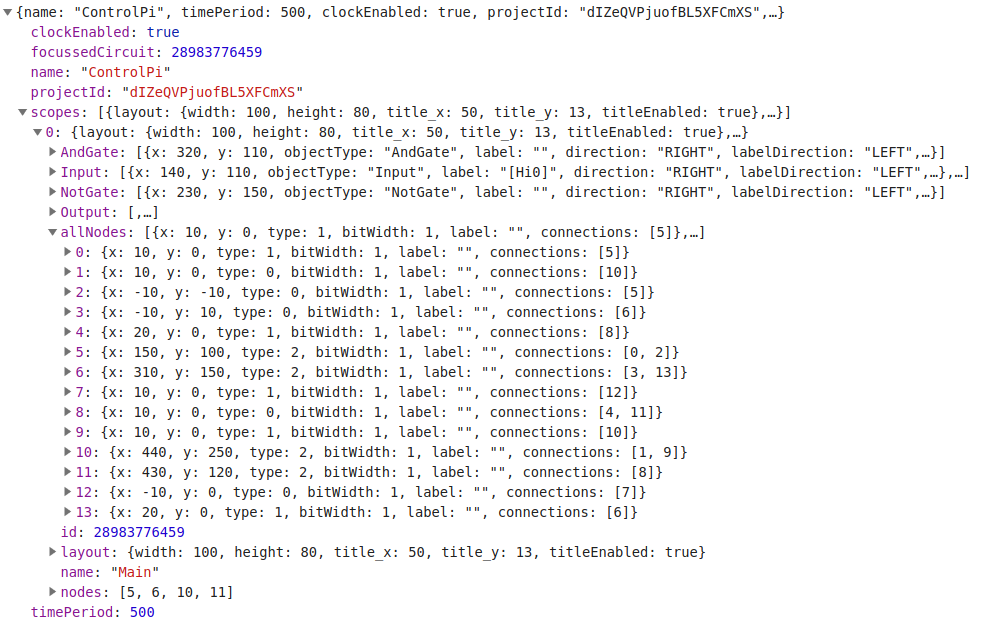
\includegraphics[width=0.8\textwidth ,clip]{./images/circuitverseLogicJson.png}
 		\caption{Darstellung der JSON Datenstruktur}
 		\label{img:circuitVerseJson}
 	\end{center} 
 \end{figure}	
 
 \begin{figure}[H]
 	\begin{center}
 		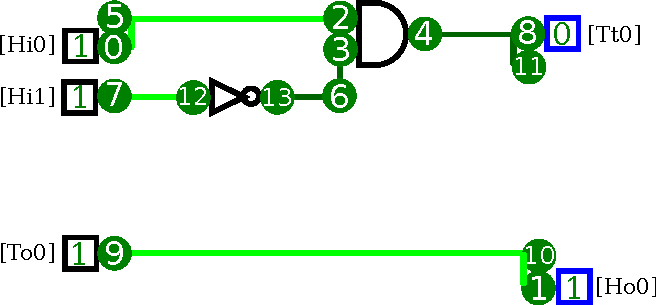
\includegraphics[width=0.65\textwidth ,clip]{./images/circuitverseLogicNodes.pdf}
 		\caption{Logikschaltung mit gekennzeichneten Knoten}
 		\label{img:circuitVerseNodes}
 	\end{center} 
 \end{figure}	
 
 
 In der vorangehenden Abbildung \ref{img:circuitVerseNodes} ist zu sehen, dass jedes Bauteil einen oder mehrere Knoten Besitzt. In \autoref{img:circuitVerseJson} ist zu sehen, dass jeder dieser Knoten eine eigene Zeile unterhalb von \texttt{allNodes} besitzt. Hieraus geht hervor, mit welchen anderen Knoten er verbunden ist. Außerdem verbirgt sich im Feld \texttt{Typ}, die Information ob es sich um einen Ausgangsknoten einen Eingangsknoten oder einen Verbindungsknoten handelt. Ist der Knoten vom Typ Eingangknoten oder vom Typ Ausgangsknoten so gehört er einem Bauteil wie einem Logikgatter, einem Eingangsbausteinen oder einem Ausgangsbausteinen. Die Anordnung der Knoten ist logischer weise anders herum wie die der Bauteile, so besitzt ein Ausgangsbaustein genau einen Eingangsknoten (z.B.  \ref{img:circuitVerseNodes} Knoten 1), sowie ein Eingangsbaustein über einen Ausgangsknoten verfügt (z.B. \autoref{img:circuitVerseNodes} Knoten 9). Ein Gatter hingegen hat einen Ausgangsknoten sowie einen oder mehrere Eingangsknoten. (z.B. \autoref{img:circuitVerseNodes} Eingangssknoten 3,4 und Ausgangsknoten 4) Für die Umwandlung in Textform schien es am sinnvollsten an einem Ausgang anzusetzen und eine Wegfindung durchzuführen, welche beim Erreichen eines Eingangsbausteins einen Endpunkt hat. Dazu durchläuft der in \autoref{img:circuitVersePAP} gezeigte rekursive Algorithmus den Weg von einem Ausgangsknoten bis zu einem Eingangsknoten. Ist ein Eingangsknoten erreicht, so wird geprüft ob es sich um den Ausgang eines Eingangsbausteins handelt, oder um den Ausgang eines Logikgatters. Da CircuitVerse die Knoten jedoch nicht nach der Art des zugehörigen Bauteils, sondern nur in Eingangsknoten Ausgangsknoten oder Leitungsknoten unterteilt, muss die in \ref{img:circuitVerseJson} gezeigte Struktur oberhalb der Eigenschaft \texttt{allNodes} vorab durchlaufen werden. Hierbei wird ein Lookup Array angelegt (siehe \autoref{img:circuitVerseLookup}), welches die Bauteile mit der Knotennummer ihres Ausgangs indiziert. Bezogen auf das in \autoref{img:circuitVerseNodes} gezeigte Beispiel, würde für das AND-Gate ein Eintrag mit dem Index 4 angelegt. \autoref{img:circuitVerseLookup} Zeigt den Eintrag für dieses AND-Gate in der aufgeklappten Zeile mit dem Index \texttt{4}. Das Array \texttt{nodesIn} beinhaltet die Knoten 2 und 3. An diesem Punkt, ruft die Funktion zur Wegfindung sich nun selbst auf. Auf diese weise werden sämtliche Logikgatter durchlaufen. In diesem Beispiel (siehe \autoref{img:circuitVerseNodes}) würde die Wegfindung von Knoten 2 über Knoten 5 auf Knoten 0 Treffen. Dieser ist jedoch kein Gateknoten sondern der Knoten eines Eingangsbausteines: Ein Endpunkt ist erreicht, das heißt es wird nun die Zeichenkette \texttt{[Hi0]} zurückgegeben. Zurück im vorher besprochenen AND-Gate, wird diese Zeichenkette nun mit dem Rückgabewert des Stranges an Knoten 3 und einem Kaufmännischen und (\&) verkettet. Da das And Gate genau zwei Eingangsknoten hat, sind nunmehr alle Knoten abgearbeitet und der Baustein gibt die Zeichenkette \texttt{[Hi0] \& ![Hi1]} zurück. Im Eingangsknoten wird diese Zeichenkette nun um den Bezeichner ergänzt.  Somit ergibt sich \texttt{[Tt0]=[Hi0] \& ![Hi1]} als Gesamtergebnis. 
  \begin{figure}[H]
 	\begin{center}
 		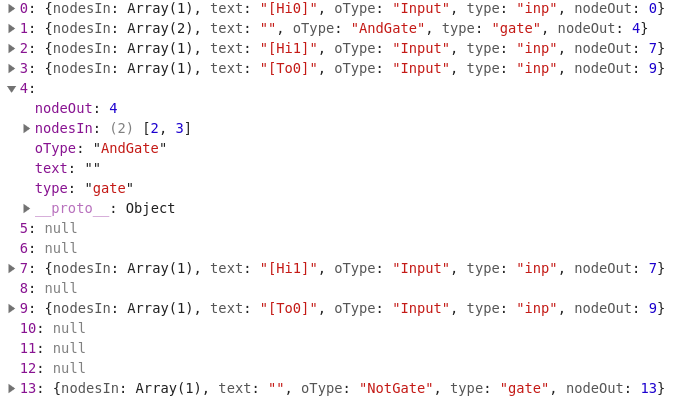
\includegraphics[width=0.65\textwidth ,clip]{./images/circuitverseLookup.png}
 		\caption{Lookup Array}
 		\label{img:circuitVerseLookup}
 	\end{center} 
 \end{figure}	
 
   \begin{figure}[H]
 	\begin{center}
 		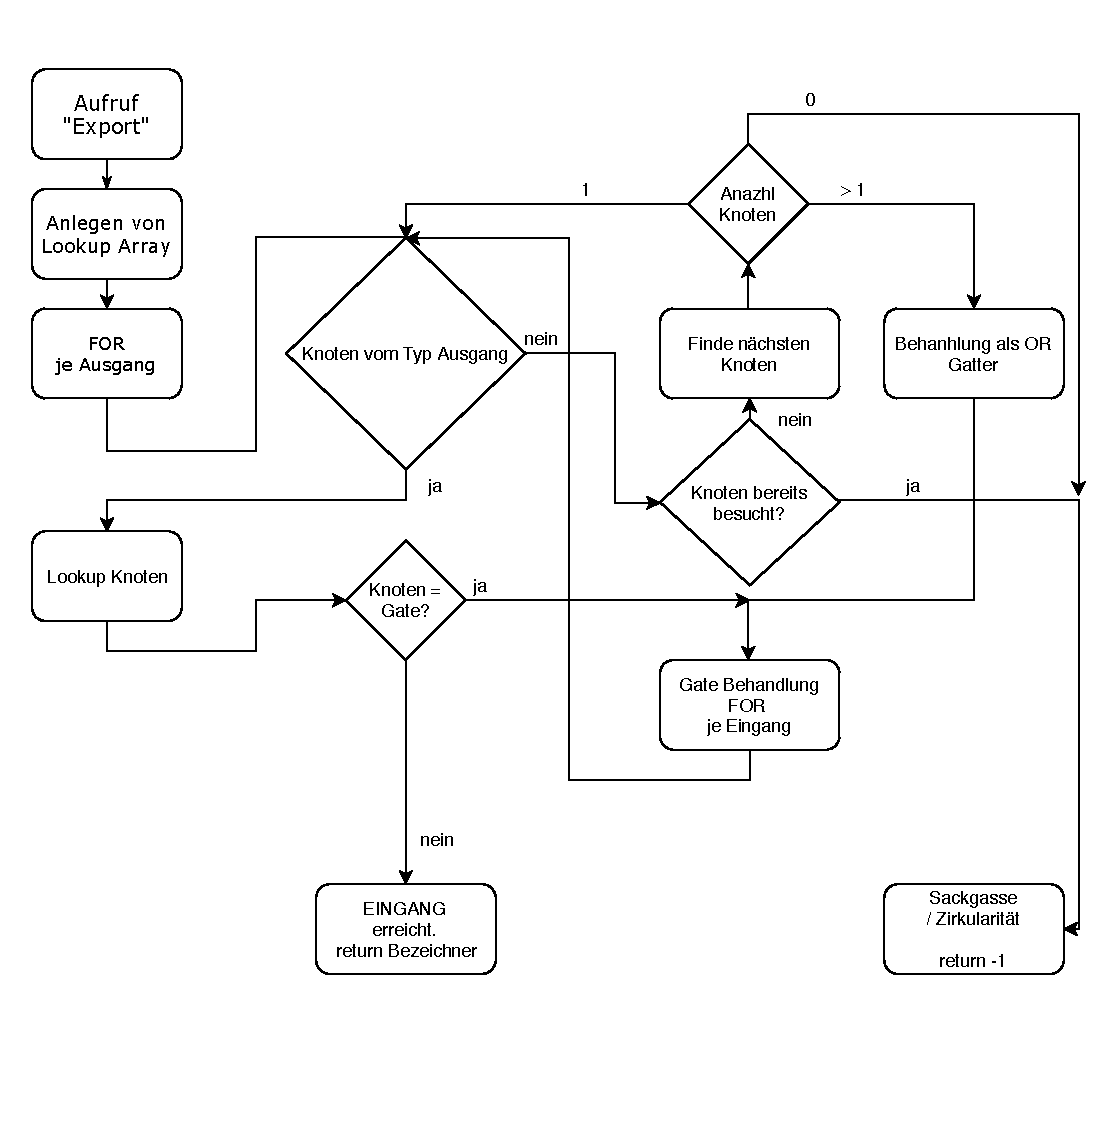
\includegraphics[width=0.75\textwidth ,clip]{./images/PAP7.pdf}
 		\caption{Programm Ablaufplan}
 		\label{img:circuitVersePAP}
 	\end{center} 
 \end{figure}
 
 \paragraph {Anpassung der Eingangsbausteine}
 
 Wie in \chphl{\ref{par:erw} \nameref{par:erw}} besprochen, wurde CircuitVerse um einen Algorithmus zum Export der gezeichneten Schaltung erweitert. Dieser wird über einen neuen Menüpunkt (siehe \ref{img:circuitVerseBright}) gestartet und zeigt dann wie in \autoref{img:circuitVerseBrightPrompt} zu sehen, das Exportergebnis zur Überprüfung an. Nach der Bestätigung des Ergebnisses wird dieses per Ajax Aufruf an ein in \autoref{kap:ums:adapterphp} näher beschriebenes PHP Script übergeben, welches es dann als Textdatei speichert. Der Menüpunkt \texttt{Save Online} schreibt das bisherig verwendete JSON Format über die selbe Schnittstelle in eine weitere Textdatei auf dem Server. Dabei wird zudem eine Abbildung der Schaltung erzeugt und ebenfalls auf den Server übertragen. Letztlich dient die Schnittstelle auch dem lesenden Zugriff auf die JSON-Datei. Sie wird beim ersten Aufruf des Logikeditors somit vom Server heruntergeladen. Damit kann die bereits vorhandene Steuerung erweitert oder verändert werden. Um zu vermeiden dass sich die Logik in der JSON Datei von der Logik in der vom Backend lesbaren Logikdatei unterscheidet, soll die Speicherung in einen Menüpunkt zusammengeführt werden. Dies dient vor allem auch dem einfacheren Verständnis durch den Endbenutzer. Es schränkt jedoch die Möglichkeit ein, neben der Steuerung die gerade \gqq{in Betrieb} ist, weitere alternative Steuerungsprogramme abzuspeichern.

\begin{figure}[H]
	\begin{center}
		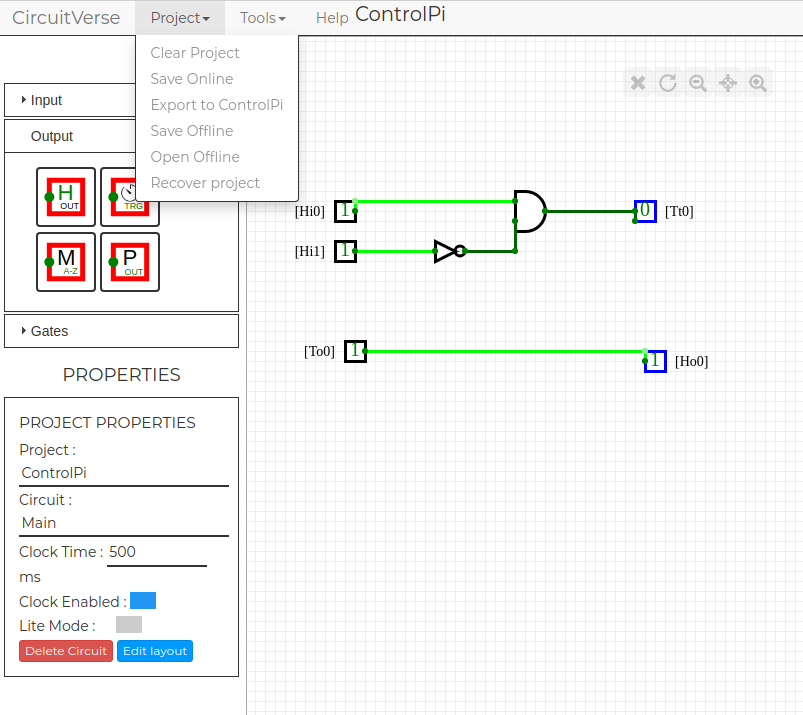
\includegraphics[width=0.75\textwidth ,clip]{./images/circuitverseLogicBright.png}
		\caption{Umgestatletes CircuitVerse}
		\label{img:circuitVerseBright}
	\end{center} 
\end{figure}

\begin{figure}[H]
	\begin{center}
		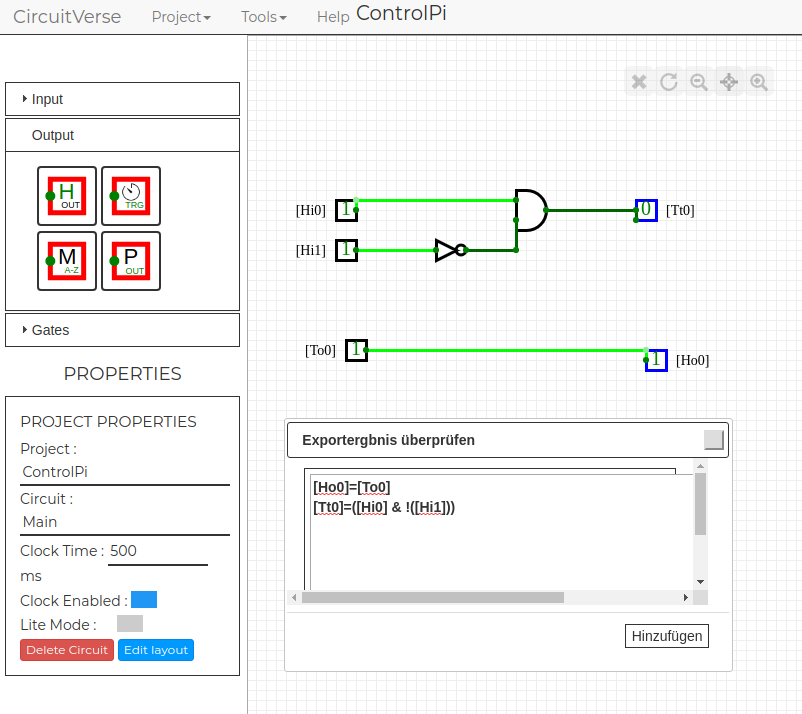
\includegraphics[width=0.75\textwidth ,clip]{./images/circuitverseLogicBrightPrompt.png}
		\caption{Dialog mit Exportergebnis}
		\label{img:circuitVerseBrightPrompt}
	\end{center} 
\end{figure}




\subsubsection{PHP Adapter Programme}\label{kap:ums:adapterphp}
\paragraph{Schnittstelle zum Speichern als Datei}\label{par:saveFile}
Da CiruitVerse als JavaScript Anwendung im Browser ausgeführt wird und somit keinen direkten Zugriff auf das Dateisystem des Servers hat, ruft es beim Speichern oder beim Laden per Ajax eine URL auf. Um Dateien nun persistent in das Dateisystem des Servers ablegen zu können wird eine API Schnittstelle benötigt, welche über ein rudimentäres PHP-Skript \texttt{logicUpdateApi} realisiert wurde. 
Dies geschieht über ein anderes PHP Skript, welches  ebenfalls über eine Ajax Anfrage angesprochen wird. Außerdem ließt dieses Script ebendiese Datei, wenn es beim Laden dieser CircuitVerse Version über JavaScript mittels Ajax aufgerufen wird. Zwischen lesendem und schreibendem Zugriff wird über die Verwendete Zugriffsmethode unterschieden, wobei \texttt{POST} einen schreibenden Zugriff gewährt und \texttt{GET} den Inhalt der Datei ließt. Da der Logikeditor in ein Helles Template eingebettet werden soll, wurde außerdem das Farbschema und die Schriftart modifiziert. 

\paragraph{WebSocket Adapter}
Das im letzen Abschnitt \ref {par:saveFile} beschrieben Verfahren zum Ablegen von Konfigurationsdaten ist ein einmaliges Ereignis, dementsprechend wird hier auch eine normale HTTP Anfrage eingesetzt, welche nach vollständiger Übertragung abgebaut wird. Im Unterschied dazu wird für die Ansteuerung der Virtuellen Kanäle sowie für die Statusabfrage der Phsyikalischen ein und Ausgänge eine persistente Verbindung aufgebaut. Dabei baut der Client eine Verbindung zu dem WebSocker Server auf welcher in Kapitel \ref{chp:ums:websockserver} näher beschrieben wird. Um duch einmalige Ereignisse von externen Diensten per HTTP zu ermöglichen, baut ein PHP Script nun \texttt{on-demand} eine WebSocket Verbindung zu dem im Backend *REF* integrierten Server auf, setzt den gewünschten Befehl um und baut die Verbindung daraufhin wieder ab. 

\subsubsection{IFTTT}




\clearpage



    \section{Übersicht Gesamtsystem}\label{kap:ausw}
 \subsection{Inbetriebnahme}
 \subsubsection{Hardware Voraussetzungen}
 Voraussetzung für den Betrieb ist ein Raspberry Pi 2 oder 3. Außerdem ist eine Erweiterungsplatine \chphl{PiFace Digital2 \cite{URL:PiFaceDigital2}} erforderlich. Diese muss vor dem ersten Start auf die GPIO-Kontakte des Raspberry Pi aufgesteckt werden. Eine Funktion ohne das Hardwaremodul ist Grundsätzlich möglich, jedoch scheint ein Betrieb ohne Hardwareschnittstelle ohne Sinn. Die Software ist so konzipiert, dass auch andere Hardware-Module denkbar sind, eine Implementierung hierfür fehlt jedoch bislang.     
 \subsubsection{Software Voraussetzungen}
 Für den Betrieb wird ein Linux Betriebssystem vorausgesetzt. Hierfür kann das angepasstes Raspbian \cite{URL:Raspian} Image genutzt werden, welches auf der beigelegten DVD zu finden. Falls auf der SD Karte bereits ein Linux Betriebssystem installiert ist, kann das Arbeitsverzeichnis des Projekts auch einfach auf den Raspberry Pi übertragen werden. Ein Git Auszug hiervon ist ebenfalls auf der beigelegten DVD. Sollte die Wahl der Distribution auf eine andere als Raspbian Strech \cite{URL:Raspian} fallen, so muss das Projekt aus den Quellen übersetzt werden. In jedem Fall ist es nötig dass SPI aktiviert wird. Dies geschieht am einfachsten über das Raspberry Pi Konfigurationsprogramm.  \texttt{sudo raspi-config} siehe \cite{URL:EnableSPI}.  
 \subsubsection{Kompilieren des Projekts}
 Ein kompilieren des Projekts ist nur erforderlich, wenn das Projekt auf einem anderen Betriebssystem als Raspbian Strech \cite{URL:Raspian} verwendet werden soll, oder wenn Änderungen am Quellcode vorgenommen werden sollen. Dafür muss zunächst eine SSH Verbindung zum System herstellt werden. Das Projekt sollte daraufhin auf das System übertragen werden. Die empfohlene Vorgehensweise hierfür ist, das GIT Repository über eine aktive Internetverbindung auf den Rasperry Pi zu klonen. \texttt{git clone https://github.com/dajuly20/ControlPi}. Um dann alle Abhängigkeiten automatisch zu installieren, kann das nachfolgend genannte Installationsscript verwendet werden: \texttt{./start\_pull\_and\_build.sh}. Sollte keine Internetverbindung bestehen, können die auf der DVD mitgelieferten Bibliotheken auch manuell installiert werden. 
 Eine Liste der benötigen Abhängigkeiten findet sich im \nameref{chp:anhang} in \autoref{chp:anhang}.  
 \subsubsection{Inbetriebnahme unter Raspbian Strech}
 Sollte auf dem Raspberry Pi bereits ein Version von Raspbian in der Version Strech installiert sein, so genügt es den Projektordner auf den Raspberry Pi zu übertragen. Hierfür dient entweder der Ordner \texttt{ControlPi} auf der beigelegten DVD, oder das GIT Repository des Projekts, welches mittels  \texttt{git clone https://github.com/dajuly20/ControlPi} auf den Raspberry Pi übertragen werden kann. Um sicherzustellen dass es sich um die aktuellste Version handelt, sollte das Projekt mit \texttt{git pull} auf den neusten Stand gebracht werden. Daraufhin kann mit \texttt{./start\_manual.sh} die Funktion überprüft werden. Dabei sollte der Benutzer in den Gruppen \texttt{spi} sowie \texttt{gpio} sein. Letztlich sollte das Projekt als Systemservice eingerichtet werden. Hierfür ist das Script \texttt{./start\_as\_service.sh} dienlich. Es wird hier neben dem eigenen Systemservice auch ein Apache2 Webserver mit in Betrieb genommen.
 
 \subsection{Inbetriebnahme mit Systemabbild}
 Auch befindet sich ein vollständiges Systemabbild \cite{URL:Image} auf der beigelegten DVD. Dieses sollte zunächst mit \texttt{tar -xvzf ControlPi-Raspbian-Strech.tar.gz} entpackt werden. Die enthaltene \texttt{.img} Datei belegt ca. 7,3 GB. Eine Speicherkarte sollte also mindestens 8 GB besser jedoch 16 GB Platz bieten. Das Systemabbild kann mit \texttt{sudo dd if=ControlPi-Raspbian-Strech.img of=/dev/<XXX> bs=4M status=progress}, oder unter Windows mit einem entsprechenden Tool \cite{URL:Win32DiskImager} auf eine Speicherkarte übertragen werden. Nach erfolgreichem Start sollte eine der LEDs auf der PiFace Erweiterungskarte dauerhaft blinken.  
 
 \subsubsection{Ermittlung der IP - Adresse}\label{chp:ausw:ip}
 Nachdem der Systemservice läuft, muss nun ermittelt werden wie ein Zugriff auf die Weboberfläche erfolgen kann. Wenn der Raspberry Pi in ein bestehendes Netzwerk integriert wird, kann dies in der Oberfläche des verwendeten Internetrouters nachgesehen werden. Sofern dieser dies unterstützt, kann auch der Hostname des Raspberry Pi für den Zugriff verwendet werden. Der Hostname im mitgelieferten Raspbian-Image lautet \texttt{ControlPi3}. Der Standard bei einem offiziellen Raspbian Image ist \texttt{raspberrypi}. Sollte kein Zugriff auf den Internetrouter bestehen oder eine Ermittlung der IP Adresse aus sonstigen gründen nicht möglich ist, kann ein Portscan durchgeführt werden. Die Steuerung öffnet in der Standartkonfiguration die Ports 80 für HTTP, den Port 443 für HTTPS bzw. SSL und den Port 22 für SSH Zugriffe. Angenommen eigene IP Adresse (Ermittlung durch \texttt{ifconfig}) wäre 192.168.8.5 mit der Subnetzmaske 255.255.255.0 so wäre der Aufruf \texttt{nmap -p 22,80,443 192.168.8.0/24}. Sollten mehrere gefundene Geräte diese Ports als offen anzeigen, so sollten die IP Adressen dieser Geräte nacheinander im Webbrowser als URL eingetragen werden um zu überprüfen bei welcher es sich um die richtige handelt.   
 
 \subsection{Funktionstest}
 \subsubsection{Testen der Betriebsbereitschaft}
 Im Auslieferungszustand ist ein zu Testzwecken bereits ein Steuerungsprogramm enthalten. Dieses lässt die LED an Ausgang 6 durch einen sich selbst aufrufenden Timer blinken. Zudem ist in diesem Testprogramm den Ausgängen \texttt{0} sowie \texttt{1} der Wert der Eingänge \texttt{0} beziehungsweise \texttt{1} zugewiesen. Ein Drücken der in \autoref{img:PiFaceDigital2} gezeigten Taster S0 oder S1 sollte also ein Leuten der entsprechenden LED zur Folge haben. Wie auch bei den Tastern, werden die LEDs von rechts nach links durchnummeriert und sind den jeweiligen Ausgängen örtlich zugeordnet. Da an den Ausgängen \texttt{0} und \texttt{1} zudem Relais angeschaltet sind, sollte sich ein Zustandswechsel auf einem dieser Ausgängen außerdem in Form eines Klickgeräusches akustisch bemerkbar machen. 

 
 \begin{figure}[H]
 	\begin{center}
 		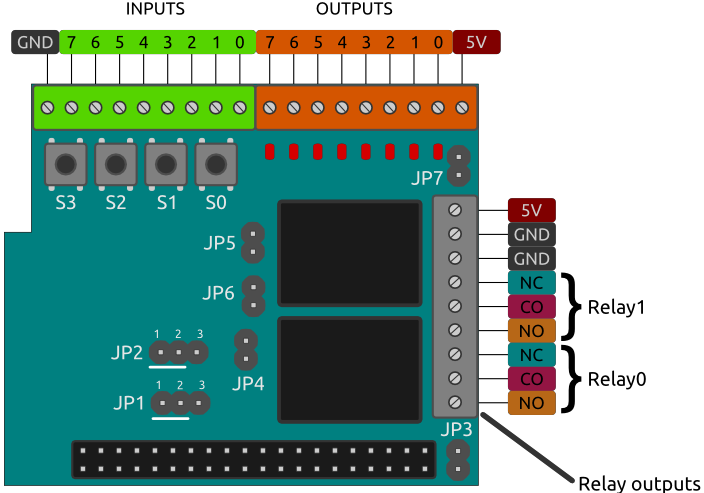
\includegraphics[width=0.95\textwidth]{./images/pifacedigital2_diagram.png}
 		\caption[Darstellung eines PiFace Digital 2]{Darstellung eines PiFace Digital 2 \cite{URL:Pfd}}
 		\label{img:PiFaceDigital2}
 	\end{center} 
 \end{figure}	

 \subsubsection{Aufruf der Weboberfläche}\label{chp:FrontendUebersicht}
Ist der Hostname oder die IP Adresse des Raspberry Pi ermittelt (siehe Abschnitt \ref{chp:ausw:ip} \nameref{chp:ausw:ip}), kann dieser im Internetbrowser aufgerufen werden. Bei Verwendung des beigelegten Raspbian Images wäre der Aufruf \texttt{http://ControlPi3}. \autoref{img:FrontendUebersicht} zeigt die Übersichtsseite der Steuerung. In der Mitte befindet sich eine Abbildung vom aktuell verwendeten Steuerungsprogramm, während an den Seiten die Zustände ein und Ausgänge angezeigt werden. Die Drop-Down Menüs oberhalb, ermöglichen es die gewünschte Ein- bzw. Ausgangsentität auszuwählen. Handelt es sich bei der ausgewählten Entität um einen Eingang, so wird anstelle einer LED ein Taste eingeblendet. Der Zustand kann dann, bei entsprechender Berechtigung (siehe \chpref{chp:ums:websock:auth} ), durch anklicken verändert werden.  

 \begin{figure}[H]
	\begin{center}
		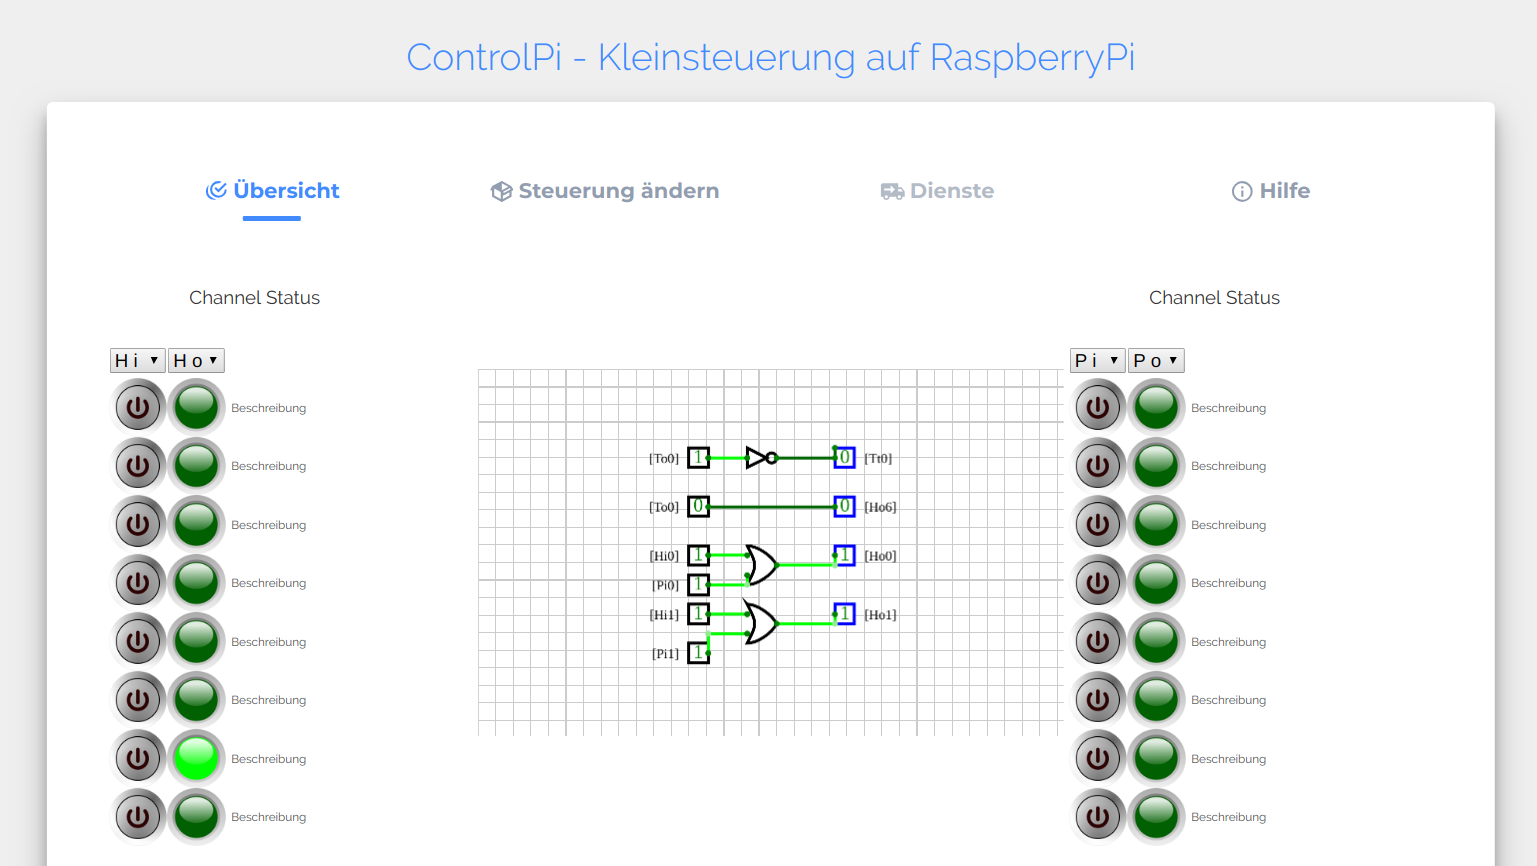
\includegraphics[width=0.95\textwidth]{./images/FrontendUebersicht.png}
		\caption{Darstellung Frontend Übersicht}
		\label{img:FrontendUebersicht}
	\end{center} 
\end{figure}

\subsubsection{Erstellen eines Steuerungsprogramms}

Um ein Steuerungsprogramm zu erstellen, muss zunächst der Tab \texttt{Steuerung ändern} angewählt werden. Nun erscheint der in \autoref{img:FrontendAenderung} abgebildete Logik-Editor CicuitVerse \cite{URL:CircuitVerse}. Sollte die vorhandene Logikschaltung nicht sofort sichtbar sein, muss die Zeichenfläche zuerst durch klicken auf das Fadenkreuz-Symbol in den Mittelpunkt gerückt werden. Soll nun eine komplett neue Schaltung gezeichnet werden, kann die Zeichenfläche durch den Unterpunkt \texttt{Clear Project} im Drop-Down Menü \texttt{Project} bereinigt werden. Alle verfügbaren Bauteile befinden sich im Bauteil-Menü auf der linken Seite. Dieses ist in die Kategorien \texttt{Input} \texttt{Output} und \texttt{Gates} unterteilt, welche sich durch anklicken aufklappen lassen. Möchte man ein Bauteil auf die Zeichenfläche schieben, so muss dieses angeklickt und der Cursor auf die Zeichenfläche bewegt werden. Ein erneutes Klicken lässt das Bauteil an der gewählten Position fallen. Die Bauteile werden schließlich mittels Drag \& Drop mit einander Verbunden. Werden Timerbausteine angeklickt, so  lassen  sich dessen Einschalt und Ausschalt- Verzögerungszeiten im Menü \texttt{Properties} einstellen. Es gilt zu beachten, dass Ausgänge jeweils nur einmal vorkommen dürfen. Gibt es mehrere Möglichkeiten in denen ein Ausgang aktiv werden soll, empfiehlt sich die Verwendung eines Und- bzw. Oder- Gatters. Nach Vollendung des Steuerungsprogramms, kann die Steuerung mit dem Menüpunkt \texttt{Save \& Export}, welcher sich im Menü \texttt{Project} befindet, übernommen und getestet werden. Eine Überprüfung auf Richtigkeit des Steuerungsprogramms erfolgt nicht. Deshalb sollte der Info-Kasten \texttt{Backend Status} im Auge behalten werden. Falls ein Fehler mit dem Steuerungsprogramm auftritt, wird dieser dort angezeigt. 
	

 \begin{figure}[H]
	\begin{center}
		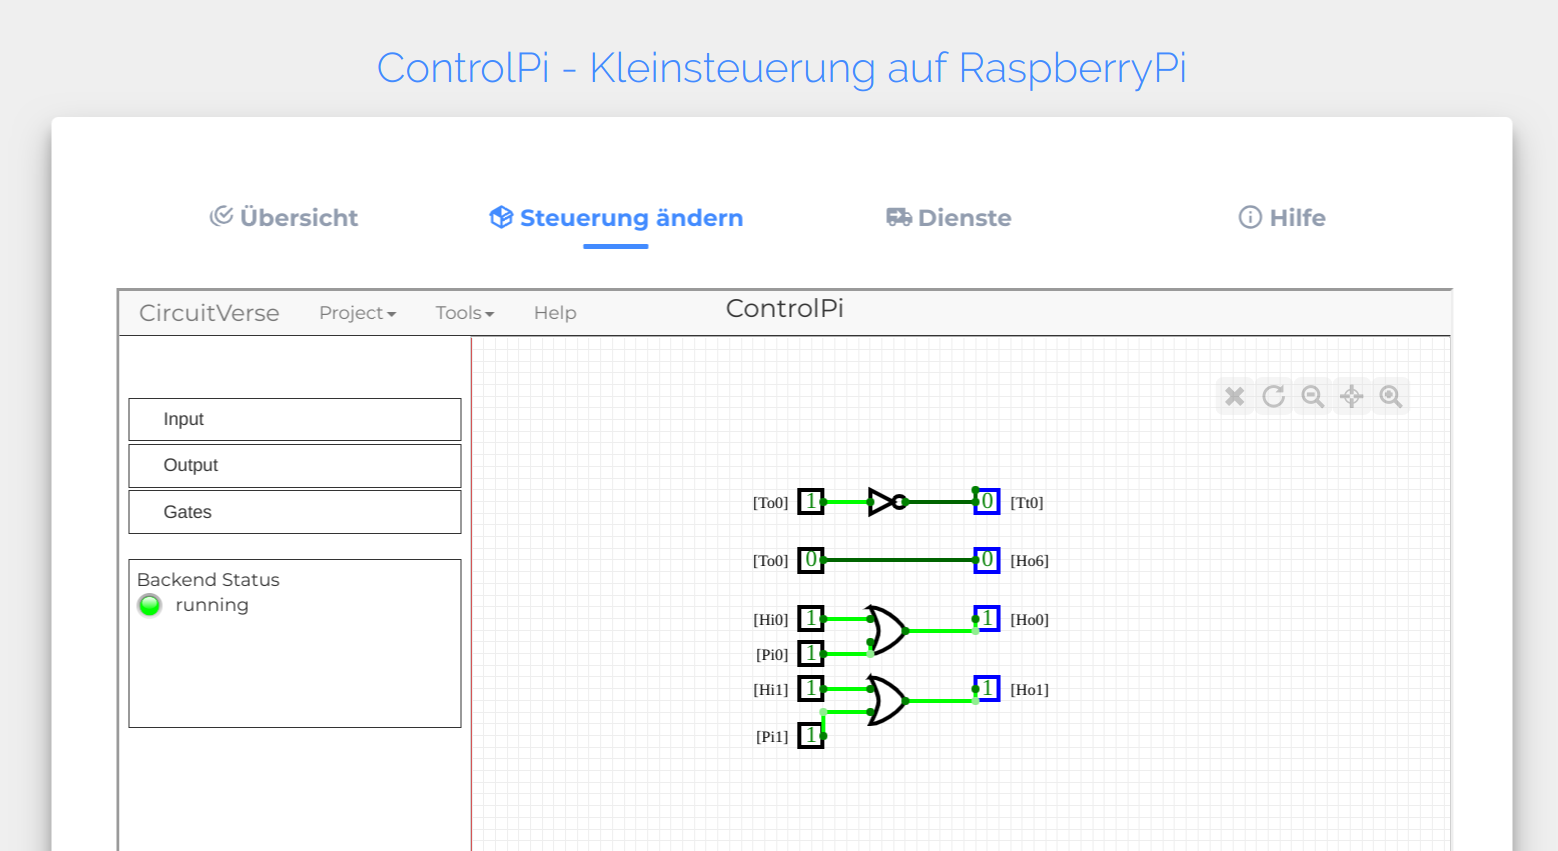
\includegraphics[width=0.95\textwidth]{./images/FrontendAendern.png}
		\caption{Darstellung Logik Editor}
		\label{img:FrontendAenderung}
	\end{center} 
\end{figure}	

\subsection{Langzeittest}
Um zu Testen wie sich die Steuerung längerfristig verhält wurde ein Timerbaustein verwendet, welcher sich selbst nach Ablauf schaltet und somit oszilliert. Als Testzeitraum wurde 48 Stunden gewählt. Dabei ließ sich feststellen, dass die Steuerung auch nach Ablauf dieser Zeit ohne Fehler weiterhin blinkte. Eine Recherche nach Neustarts des Systemdienstes blieb ebenfalls ohne Treffer.    

 \subsection{Bugs}
 Zum derzeitigen Stand sind noch einige Probleme enthalten auf die nachfolgend eingegangen wird. Als erstes sei hier zu nennen, dass die Reihenfolge in welcher das Backend über die Zeilen des erzeugten Steuerungsprogramms Iteriert unter bestimmten Voraussetzung Probleme bereitet. So wird der Wert eines Ausgangs unter noch nicht näher bekannten Umständen erst mit der nächsten Iteration des Logikprogramms übernommen. Dies könnte durch generelles doppeltes iterieren behoben werden, was allerdings die Performance vermindert. Der Logikeditor in der Benutzeroberfläche hat ebenfalls ein Darstellungsproblem welches bislang noch nicht behoben werden konnte. Beim Aufruf wird die bereits vorhandene Logikschaltung nicht Automatisch zentriert, sondern ist beinahe unsichtbar in der oberen linken Ecke der Zeichenfläche. Ein klicken auf das Fadenkreuz-Symbol bringt hier Abhilfe.  
 
 \subsection{Fazit}
 Das Projekt teilte sich wesentlich in zwei Teile. Das Backend ist einen Teil, welcher sich auf einer sehr Hardwarenahen Ebene abspielte. Die Benutzeroberfläche hingegen, ist sehr nahe am Benutzer. Damit spiegelte dieses Projekt viele Nuancen der Technischen Informatik wieder. Die meiste Arbeit entfiel dabei in die Programmierung des Backend, dass in mehrere parallele Handlungsstränge aufgeteilt ist, welche synchronisiert werden wollen. Auch das arbeiten mit C++ Bibliotheken und das Kompilieren brachte einige Herausforderungen mit sich. Die Anbindung der Benutzeroberfläche beleuchteten eine relativ junge Technologie der modernen Webentwicklung. Auch das Anpassen des Logik Editors und die damit verbundene Einarbeitung in ein fremdes Open-Source Projekt machten dieses Projekt sehr lehrreich. Zuletzt boten sich auch die Gelegenheit zu erproben wie eine Software durch Systemabbilder oder Git verteilt werden kann, und wie man diese mit \LaTeX\ so dokumentiert, dass möglichst alle Aspekte beleuchtet werden und die  Arbeit unkompliziert weitergeführt werden kann.
 
 \subsection{Ausblick}
 Die Steuerung funktioniert in den meisten Fällen ohne Probleme, ist jedoch noch nicht über ein frühes Betastadium hinaus. Es bedarf nun Feldtests um weitere Bugs in der Software aufzuspüren. Außerdem sind noch einige Funktionserweiterungen Denkbar. Zuerst anzuführen wäre hier die Kopplung zweier Geräte. Die Grundvoraussetzungen hierfür sind durch die Implementierung  von Websockets bereits geschaffen. Entweder müsste hier eine Mittelschicht geschrieben werden, welche die zwei Websocket Server auf den beiden Geräten miteinander kommunizieren lässt. Etwas eleganter jedoch wäre die Implementierung eines Websocket Clients in das Backend. Mit einer angepassten Konfigurationsdatei könnte das Backend sich so zu einem anderen Gerät verbinden um dessen Virtuelle Ein und Ausgänge auch am lokalen Gerät nutzbar zu machen. Websockets haben durch die persistente Verbindung sehr gutes Verhältnis zwischen Overhead und Payload und sollten somit eine recht geringe zeitliche Verzögerung ermöglichen. Die Erfahrung von der Verbindung zwischen Web-Frontend und Backend zeigen kaum merkliche Verzögerungszeiten. Eine weitere Funktion über welche nachgedacht wurde, ist ein anlegen von Unterstromkreisen. Somit könnten zum Beispiel blinker Bausteine oder \texttt{Stromstoßschalter}, das sind Bauteile die ihren Logikzustand durch einen Eingangsimpuls wechseln, realisiert werden. Dabei würde die Implementierung abstrahiert und die Übersichtlichkeit erhöht. Ebenfalls denkbar wäre die Zusammenfassung der Timer Ein- und Ausgänge in ein einziges Bauteil. Die Umsetzung beim Export könnte hierbei beibehalten werden, jedoch könnten die Timer Bausteine dann zwischengeschaltet werden, was deren Einsatz vereinfacht. 
  

 
 
\clearpage
    \section{Ausblick}\label{kap:aus}


    \clearpage                                                                      %Leere Seite
    \singlespacing
        \printbibliography                                                          %Literatur Verzeichnis
    \onehalfspacing
    \clearpage                                                                      %Neue Seite
%    \pagenumbering{Alph}                                                            %Seitenzahl aplhanumerisch
        \section{Anhang}\label{chp:anhang}
\subsection*{Inhalt der beigelegten DVD}
\begin{figure}[H]

\dirtree{%
.1 \textbackslash\textcolor{folder}{DVD}.
.2 \textcolor{folder}{ControlPi/}\DTcomment{Git-Auszug des Projektordners}.
.2  \textcolor{folder}{libmcp23s17/}\DTcomment{Git-Auszug der Bibliothek Libmcp23s17}.
.2 \textcolor{folder}{libpifacedigitalcpp/}\DTcomment{Git-Auszug der Bibliothek Libpifacedigitalcpp}.
.2 ControlPi-Raspbian-Strech{.}tar{.}gz\DTcomment{Komplettes System-Image}.
.2 Demo-Video{.}mkv\DTcomment{Demo Video mit Untertitel}.
.2 talk{.}pdf\DTcomment{Im Rahmen der Arbeit gehaltener Vortrag}.
.2 thesis{.}pdf\DTcomment{Dieses Dokument}.
}
\caption{Inhalt der beigelegten DVD}
\label{fig:cd}
\end{figure}

\subsection*{Eingesetzte Software}

In \autoref{tab:usedSoftware} werden die wichtigsten Programme, die zum Entwickeln verwendet wurden, aufgelistet.

\begin{table}[H]
\centering
\caption{Liste der eingesetzten Software}
\label{tab:usedSoftware}
\begin{tabular}{ll}
\hline
Programm       & Version      \\ \hline
CMake          & 3.13.4       \\
GCC            & 8.1.0        \\
Boost		   & 1.6.9		  \\
Boost Beast	   & 2.3.5		  \\
libmcp23s17    & 0.3.3		  \\
libpifacedigital & 3.0.1      \\
Linux Kernel   & 4.14.98      \\
Raspbian 	   & 9 (strech)   \\
Apache 		   & 2.4.25       \\
PHP			   & 7.0.33		  \\
Chromium       & 73.0.3683.86 \\
Firefox        & 66.0.3       \\

\end{tabular}
\end{table}

                                         %Anhang
\end{document}
